\documentclass[12pt,a4paper]{article}
\usepackage[german]{babel}
\usepackage[utf8]{inputenc}
\usepackage{amsmath}
\usepackage{amsfonts}
\usepackage{amssymb}
\usepackage{amsthm}
\usepackage{natbib}
\usepackage{graphicx}
\usepackage{wrapfig}
\usepackage{enumitem} 
\usepackage{subfigure} 

\usepackage{multicol}

\usepackage{fancyhdr}

\pagestyle{fancy}
\rhead{}
\lhead{\rightmark}

\author{Florian Neuweiler}
\date{}
\title{Harmonische Lage}

\begin{document}
\selectlanguage{german}

\setlength{\columnsep}{1.5cm}
\setlength{\columnseprule}{1pt}

\theoremstyle{definition}

\begin{titlepage}
\centering
{\scshape\LARGE Fachhochschule Karlsruhe - Technik und Wirtschaft \par}
\vspace{1cm}
{\scshape\Large Seminararbeit\par}
\vspace{1.5cm}
{\huge\bfseries Harmonische Lage\par}
\vspace{1.5cm}
{\Large\itshape Florian Neuweiler\par}
\vspace{1.5cm}
betreut von\par
Prof.~Dr.~rer.~nat.~Frank Schaefer
\vspace{2cm}

\vfill
{\large \today\par}
\end{titlepage}

\newpage
\tableofcontents

\newpage

\setlength{\parindent}{0pt}

\section{Einleitung}
Harmonie\dots ein Wort, mit dem wir Menschen das ausgewogene und ausgeglichene Zusammenspiel von Tönen, Verhältnissen und Maßen verstehen. Hauptsächlich verwenden wir erst dann den Begriff \glqq Harmonie\grqq ~oder bezeichnen etwas \glqq harmonisch\grqq , wenn wir von einer Regelmäßigkeit in der Anordnung einzelner Objekte sprechen, zu der wir zusätzlich einen übergeordneten Sinn oder Sachverhalt vermuten.

Betrachten wir beispielsweise einen Säulengang wie in Abbildung \ref{fig:saeulen}, so würden wir die Anordnung der Säulen zum Horizont als \glqq harmonisch\grqq ~bezeichnen. Dabei definiert die Anordnung der Säulen in unserem Bild ein bestimmtes Maß bzw.~ Netz, mit dem wir weitere Säulen harmonisch anreihen, oder zwischen zwei bereits vorhandenen Säulen platzieren können.

\begin{figure}[htbp]
\subfigure[Original]{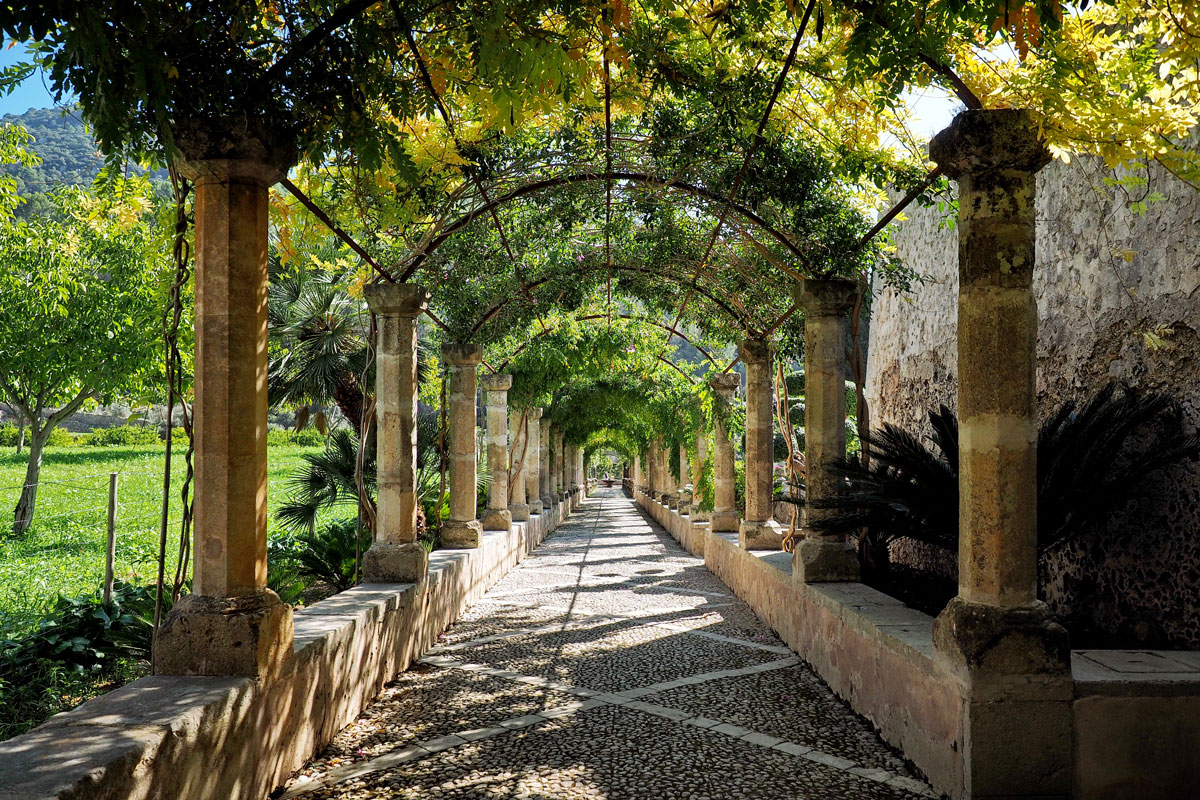
\includegraphics[width=0.45\textwidth]{Bilder/Saeulengang.jpg}} \hfill
\subfigure[Mit Netz]{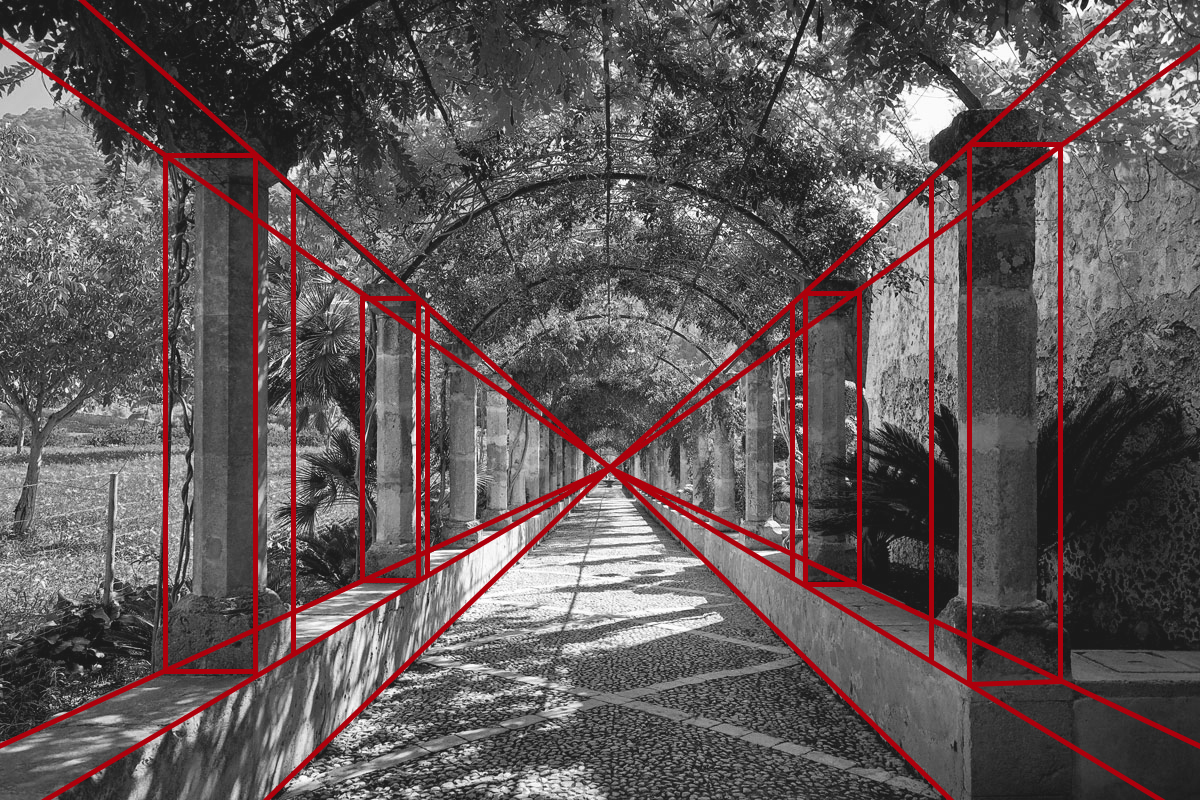
\includegraphics[width=0.45\textwidth]{Bilder/Saeulengang_Netz.jpg}}
\caption{Ein harmonischer Säulengang}
\label{fig:saeulen}
\end{figure}

Dabei fällt uns auf, wenn wir eine weitere Säule platzieren und sich demselben Maß-System wie zuvor unterordnet, dass diese die Harmonie des Bildes nicht durchbricht. Dieses Maß wird in der Mathematik als harmonische Lage bzw.~ harmonische Folge von Punkten genannt und ist das Thema der vorliegenden Arbeit.

I, Folgenden wird die harmonische Lage von Punkten und Geraden zuerst über ein geometrisches Beispiel eingeführt und später der rechnerische Zugang mithilfe des Teil- und Doppelverhältnisses beschrieben. Anschließend erweitern wir die harmonische Lage auf weitere mathematische Gebiete wie das harmonische Mittel, die harmonische Folge, sowie dem Goldenen Schnitt. Zuletzt wird die Anwendung der harmonischen Lage in der Malerei und heutigen Gestaltungsrichtlinien genauer betrachtet.

\newpage
\section{Die Harmonischen Lage}
\label{subsec:dieHarmonischeLage}

\textit{\glqq Harmonisch\grqq ~ist ein großes Wort; es bedeutet hier: Wenn die inneren und die äußeren Verhältnisse im Einklang sind. Es lohnt sich darüber nachzusinnen.} \citep[S.~53]{projektiveGeometrie}.

\begin{wrapfigure}{r}{5cm}
\centering
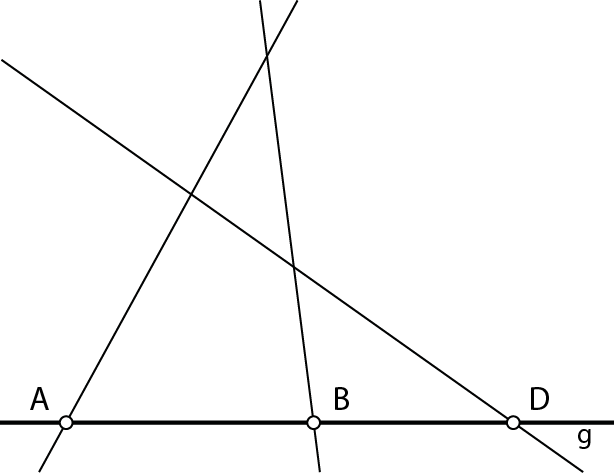
\includegraphics[width=5cm]{Bilder/herleitung1.png}

\vspace{0.5cm}
\centering
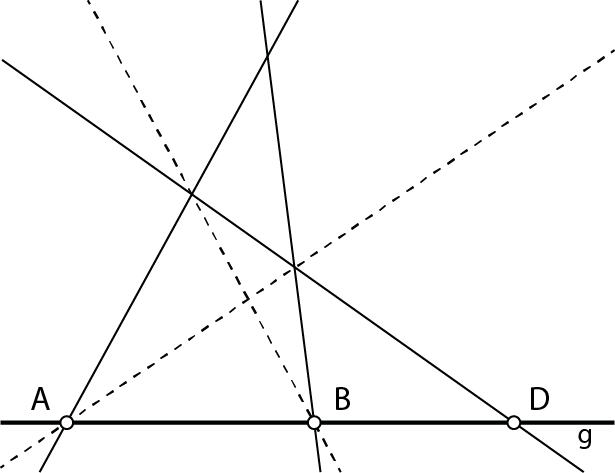
\includegraphics[width=5cm]{Bilder/herleitung2.png}

\vspace{0.5cm}
\centering
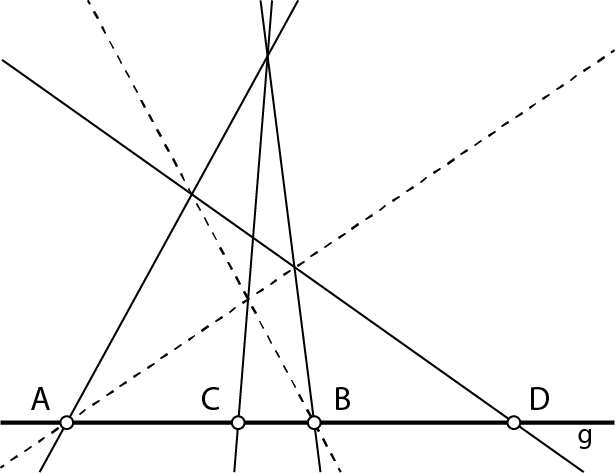
\includegraphics[width=5cm]{Bilder/herleitung3.png}
\caption{Geometrische Konstruktion der harmonischen Lage}
\label{fig:Herleitung}
\end{wrapfigure}

Tatsächlich handelt es sich bei der harmonischen Lage von Punkten und Geraden um einer der wichtigsten Begriffe der projektiven Geometrie. Ähnlich wie der Tastsinn des physischen Raumes bildet die harmonische Lage ein natürliches Maß für Bilder und dem Sehsinn. Zudem handelt es sich bei der harmonischen Lage um eine Invariante der projektiven Geometrie. Demnach bleibt die harmonische Lage bei allen projektiven Operationen erhalten, dazu aber später mehr.

Doch was genau ist die harmonische Lage wirklich? Um dies zu veranschaulichen erläutern wir die harmonische Lage anhand eines Beispiels (Abb.~\ref{fig:Herleitung}):

Betrachten wir eine Gerade $g$, auf der sich drei Punkte $A$, $B$ und $D$ befinden, die willkürlich auf dieser Geraden positioniert wurden. Aus diesen drei Punkten auf $g$ lässt sich nun eindeutig ein weiterer \glqq harmonischer\grqq ~Punkt $C$ konstruieren, der ebenso wie $A$, $B$ und $D$ auf $g$ liegt. Um diesen Punkt $C$ geometrisch zu konstruieren wird wie folgt vorgegangen:

Zunächst werden von jedem der Punkte $A$, $B$ und $D$ aus eine Gerade gezogen. Diese drei Geraden haben drei Schnittpunkte. Nun werden zwei weitere Geraden gezogen: die eine führt durch den Punkt $A$ und den Schnittpunkt der zwei Geraden durch $B$ und $D$, die andere durch den Punkt $B$ und den Schnittpunkt der zwei Geraden durch $A$ und $D$ (hier gestrichelt dargestellt).

Durch den Schnittpunkt dieser zwei soeben gezeichneten Geraden wird eine weitere Gerade gebildet, die auch durch den Schnittpunkt der zwei Geraden durch $A$ und $B$ geht. Der Punkt dieser Geraden, der auch auf der Geraden $g$ liegt, ist der von uns gesuchte Punkt $C$. Diese Konstruktion wird auch harmonische Spiegelung von $D$ an $A$ und $B$ genannt \citep[vgl.~][S.~34]{harmonischeLage}.

Egal, wie die Geraden durch $A$, $B$ und $D$ gezogen wurden, es lässt sich immer wieder denselben Punkt $C$. In anderen Worten: Der vierte Punkt $C$ ist unabhängig von der Wahl der drei Geraden durch $A$, $B$ und $D$ (Abb.~\ref{fig:AndereWahl}).

\begin{figure}[htbp]
\centering
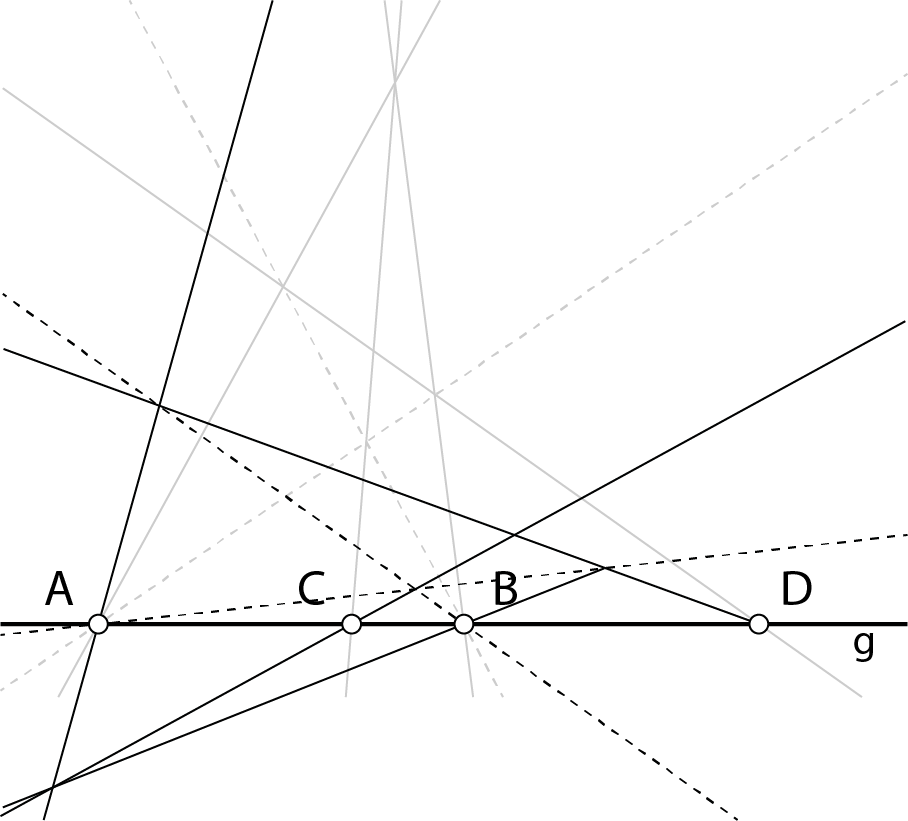
\includegraphics[width=0.5\textwidth]{Bilder/fuer_mehrere_geraden.png}
\caption{Eine andere Wahl der Geraden}
\label{fig:AndereWahl}
\end{figure}

\subsection{Definition}

Anhand des oberen Beispiels lässt sich nun im allgemeinen die harmonische Lage definieren.
\newline
\newline
\textbf{Definition von vier Punkten:}

Zwei Punktepaare $(A,B)$, $(C,D)$ auf einer Geraden $g$ \glqq trennen sich harmonisch\grqq , wenn sie so liegen wie die Ecken und die Nebenecken eines vollständigen Vierseits in einer Nebenseite.

\begin{wrapfigure}{r}{0.35\textwidth}
\centering
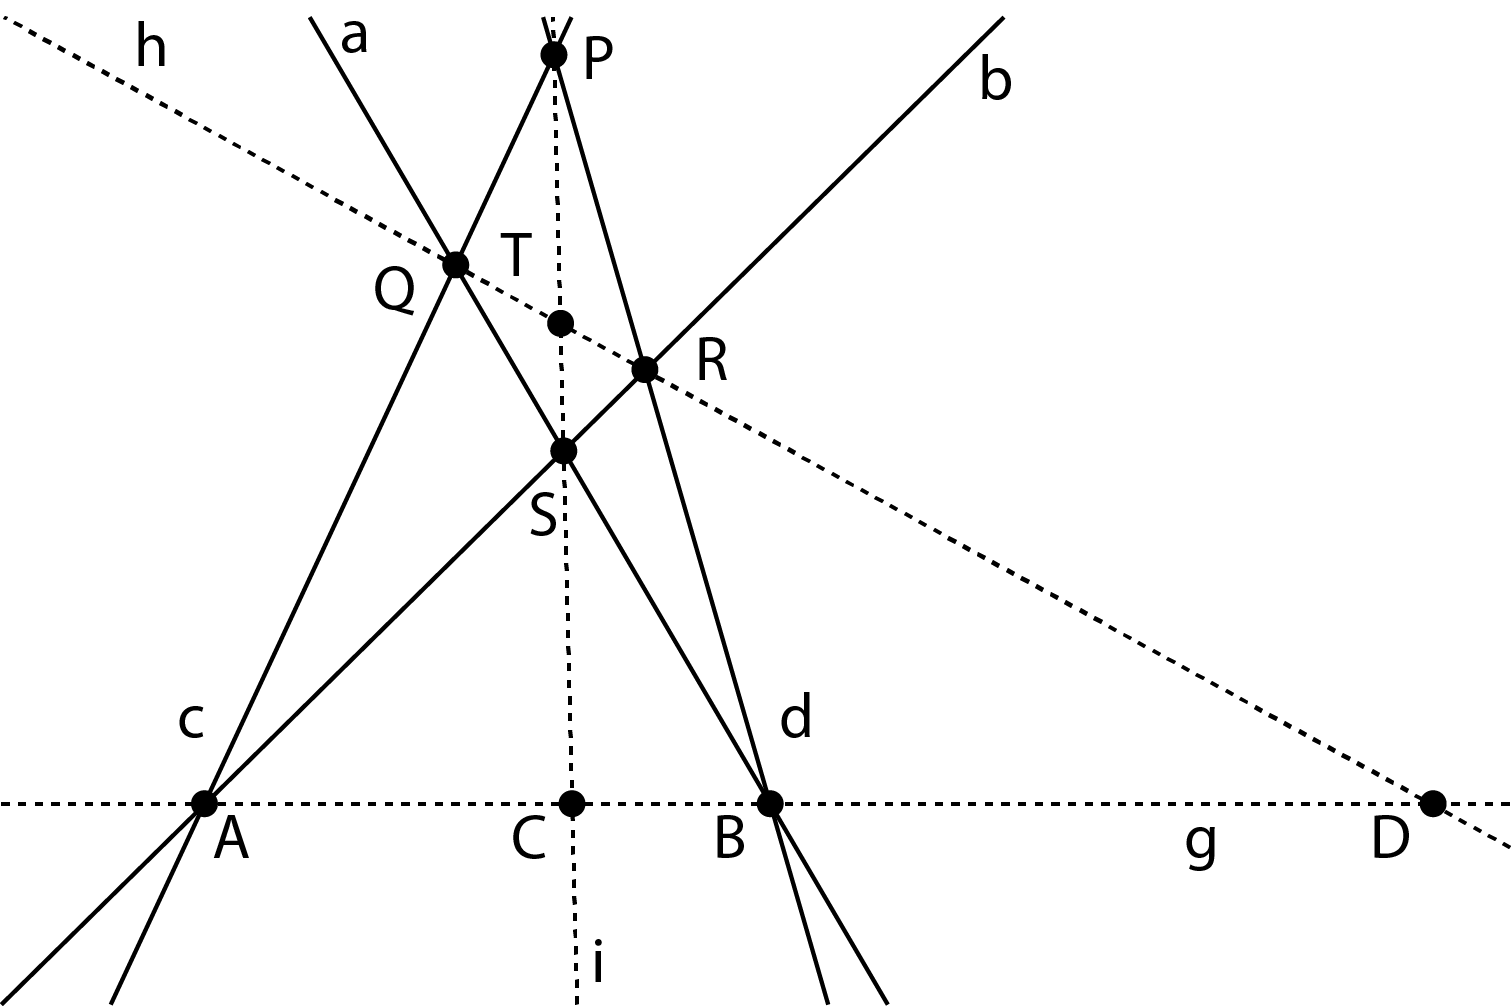
\includegraphics[width=0.35\textwidth]{Bilder/vollstaendigesVierseit.png}
\end{wrapfigure}

Dabei versteht man unter einem vollständigen Vierseit eine Figur bestehend aus den Geraden bzw.~Seiten $a$, $b$, $c$ und $d$ , den sechs Ecken, die jeweils die Schnittpunkte von je zwei Seiten sind, den drei Nebenseiten, die jene Ecken verbinden, die nicht auf den Hauptseiten liegen, sowie drei Nebenecken (gegeben durch die Schnittpunkte der Nebenseiten untereinander).
\newline
\newline
\textbf{Definition von vier Geraden:}

\begin{wrapfigure}{r}{0.35\textwidth}
\centering
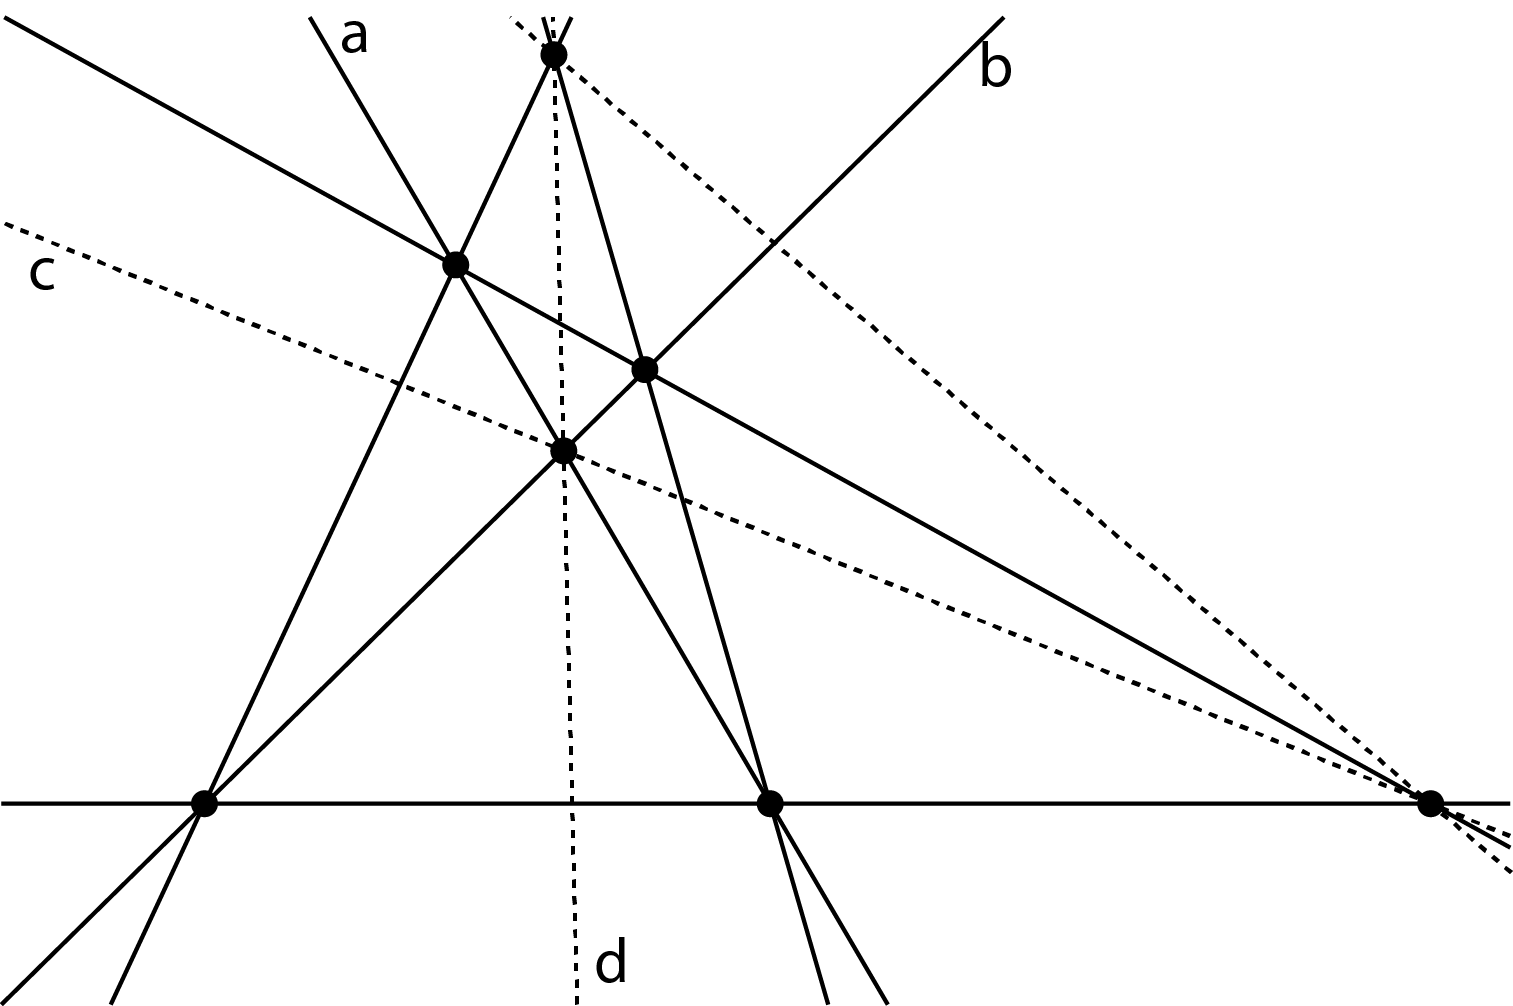
\includegraphics[width=0.35\textwidth]{Bilder/vollstaendigesViereck.png}
\end{wrapfigure}

Zwei Geradenpaare $(a,b)$, $(c,d)$ in einem Punkt $P$ \glqq trennen sich harmonisch\grqq , wenn sie so liegen wie die Seiten und die Nebenseiten eines vollständigen Vierecks in einer Nebenecke.

Dabei versteht man unter einem vollständigen Viereck eine Figur bestehend aus den Ecken $A$, $B$, $C$ und $D$ (von denen nicht drei auf einer Geraden liegen), den sechs Seiten durch jeweils zwei der Ecken, den drei Nebenecken, die als Schnittpunkte dieser Seiten hinzukommen (gestrichelt dargestellt), sowie den Nebenseiten (gegeben durch die Nebenecken).
\newline
\newline
Die Bezeichnungen \glqq trennen sich harmonsich\grqq ~ist gleichbedeutend zu den Aussagen wie \glqq liegen harmonisch zueinander\grqq , \glqq sind in Harmonischer Lage\grqq ~oder \glqq bilden einen harmonischen Wurf\grqq .
\newline
\newline
Wir können zur Konstruktion vierer harmonischer Punkte wie in unserem Beispiel vorgehen. Es existieren aber noch andere Möglichkeiten zur Konstruktion des vierten harmonischen Punktes:

\begin{figure} [htbp]
\subfigure[Thaleskreis]{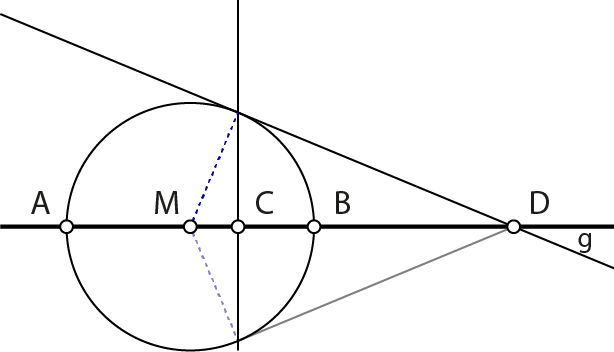
\includegraphics[width=0.4\textwidth]{Bilder/thales.png}} \hfill
\subfigure[Strahlensatz]{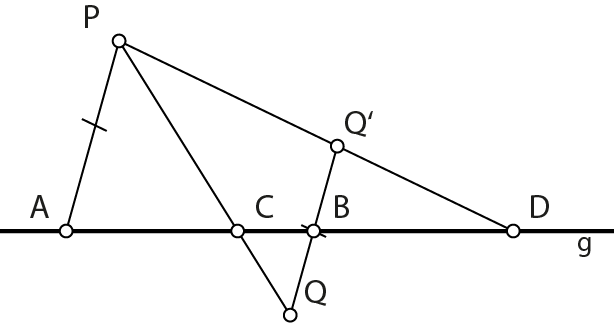
\includegraphics[width=0.4\textwidth]{Bilder/strahlensatz.png}}
\caption{Bestimmung des 4. harmonischen Punktes $D$}
\end{figure} 

\newpage
\subsection{Die harmonische 13er Konfiguration}
\label{subsec:harmonischeKonfiguration}

Wie wir schon in der Definition der harmonischen Lage gesehen haben, können sowohl Punkte als auch Geraden harmonisch zueinander liegen. Da in den Definitionen sowohl von vollständigen Vierseiten und Vierecke die rede war und sich diese geometrischen Grundgebilde aufeinander inzidieren lassen, können wir daraus eine harmonische Grundfigur, die sogenannte \glqq harmonische 13er Konfiguration\grqq bauen. Da wir sowohl ein Vierseit als auch ein Viereck diese Konfiguration beinhaltet, benötigen wir für die Konstruktion der Konfiguration insgesamt 13 Geraden und 13 Punkte - womit auch die Frage nach dem Namen geklärt wäre. Diese 13 Punkte und Geraden bilden sich zusammen

\begin{itemize}
\item[]aus den 4 Seiten und 6 Ecken des vollständigen Vierseits,
\item[]den 6 Seiten und 4 Ecken des vollständigen Vierecks und
\item[]den 3 Seiten und Ecken des gemeinsamen Nebendreiecks/-seits.
\end{itemize}

\begin{figure}[htbp]
\centering
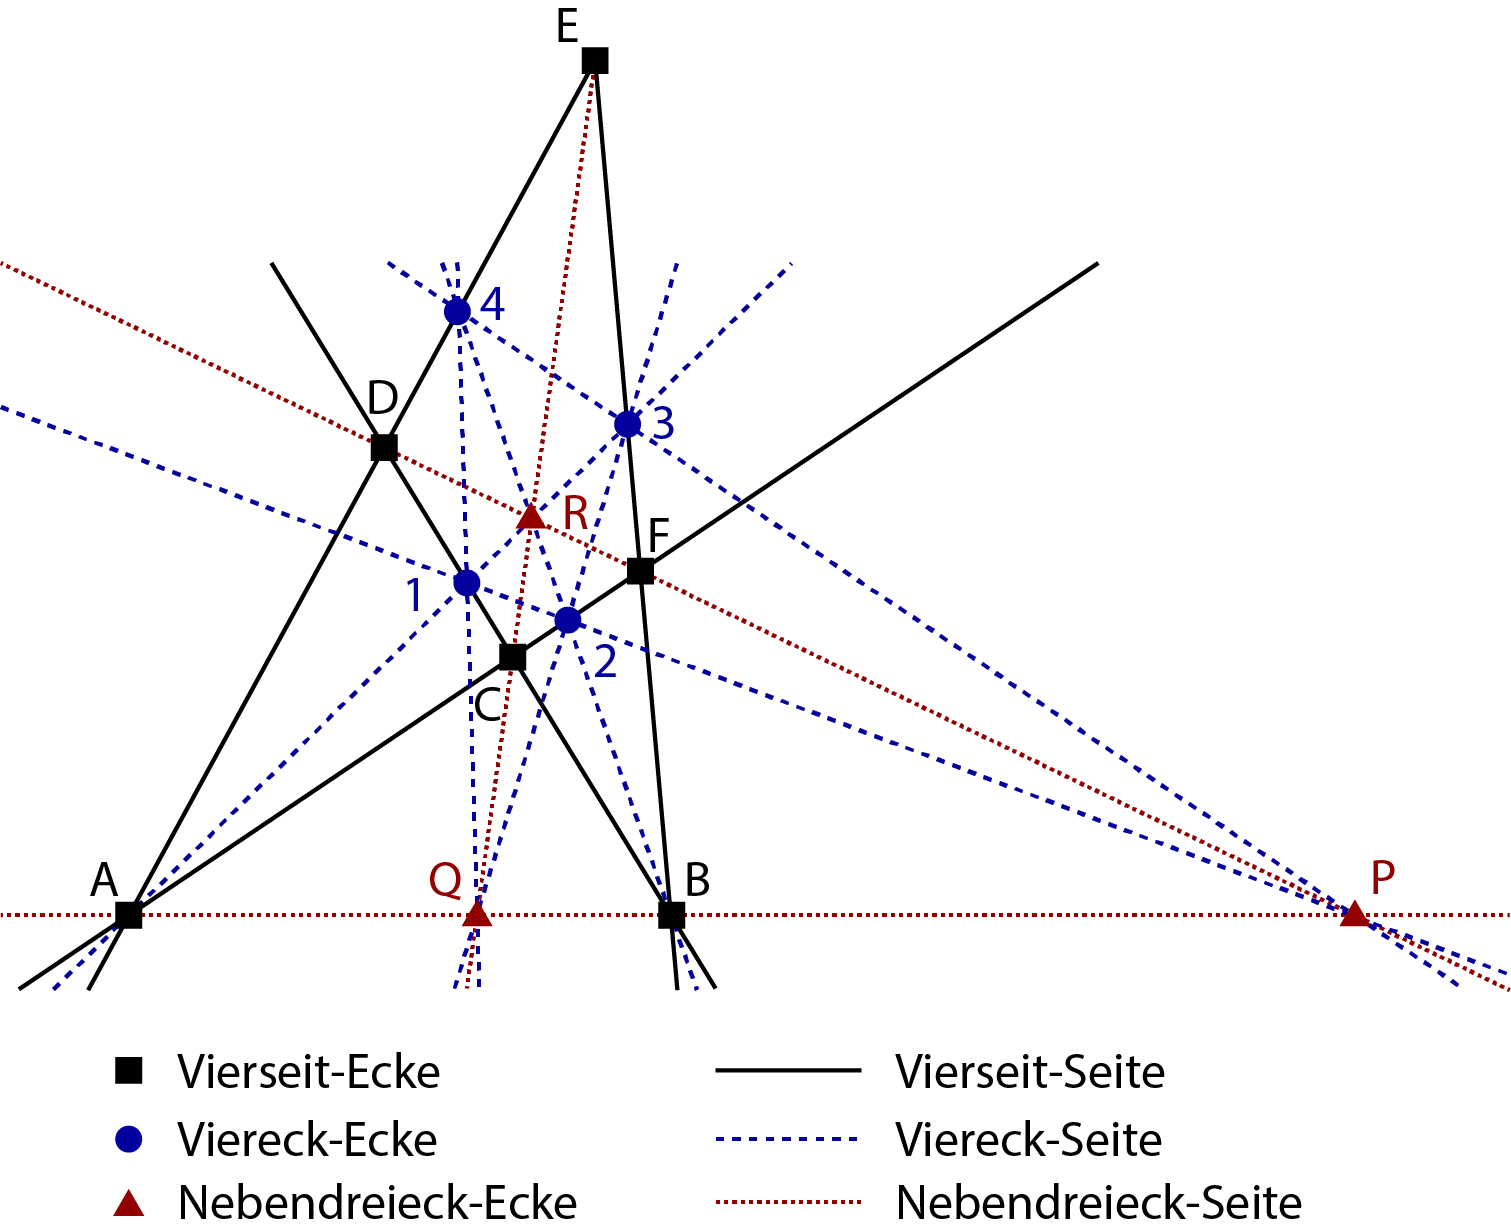
\includegraphics[width=0.7\textwidth]{Bilder/13erKonfigStepbyStep.png}
\caption{Beispiel einer harmonischen 13er Konfiguration}
\label{fig:harmFigur}
\end{figure}

Für die Konstruktion der harmonischen 13er Konfiguration wäre es am einfachsten, mit einem vollständigen Viereck bzw.~ Vierseit zu beginnen und auf dieser die weiteren Punkte und Geraden aufbauen.

\begin{wrapfigure}{r}{0.35\textwidth}
\centering
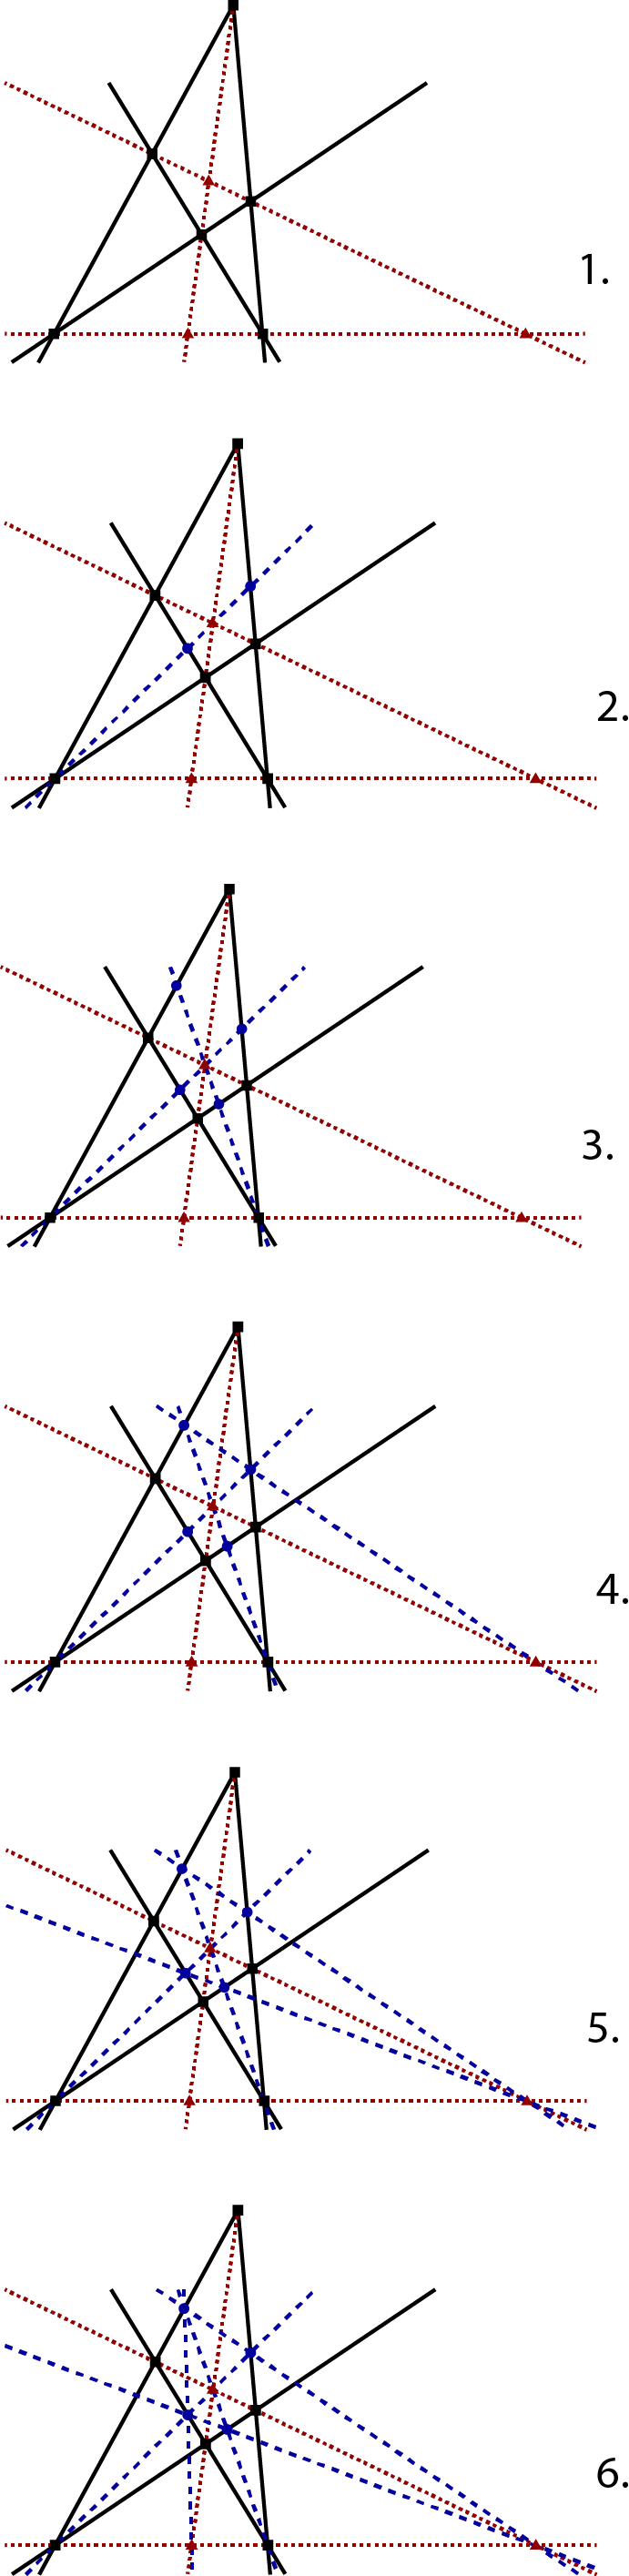
\includegraphics[width=0.35\textwidth]{Bilder/13erKonfigStepbyStep3.png}
\end{wrapfigure}

In diesem Fall entscheiden wir uns für ein vollständiges Vierseit als Grundkonstrukt. Darin wollen wir nun die Punkte und Geraden eines vollständigen Vierecks bestimmen, das dasselbe Nebendreieck hat und dessen Seiten mit den Ecken inzidieren. Dazu gehen wir wie folgt vor:

Zuerst betrachten wir die Ecken des Vierseits, in welche zwei Seiten des Vierseits und eine Seite des Nebendreiecks falle. In unserer Abbildung wären das die Punkte A, B und E. Dabei lassen wir von diesen drei Punkten die Ecke wegfallen, die mit je einer Seite des Vierseits mit den anderen Punkte verbunden ist. Hier wäre das der Punkt E, sodass wir jetzt nur noch die Ecken A und B betrachten. Von diesen zwei Ecken ziehen wir je eine Gerade aus, die sich alle in derselben Ecke des Nebendreiecks schneiden, mit der sie sich nicht auf einer Nebenseite befinden. In unserem Beispiel ist das R. Dabei bilden die Schnittpunkte der Seiten des Vierseits mit den Geraden die vier Ecken des vollständigen Vierecks, wobei die Punkte A und B nicht dazu gehören. Auch sind die von uns konstruierten Geraden die Seiten unseres gesuchten Vierecks. Schließen wir nun das Viereck, indem wir nun alle Ecken des Vierecks so miteinander verbinden, das immer zwei Ecken auf eine Seite des Vierecks fallen.
\newline
\newline
Damit hätten wir die harmonische Grundfigur geschaffen. In dieser Konstruktionsbeschreibung wurde jedoch der Beweis, dass die Seiten des Vierecks durch die Ecken des Nebendreiecks gehen müssen ausgelassen. Für eine genauere Konstruktion der harmonischen 13er Konfiguration ist \citep{projektiveGeometrie} Seite 48f zu empfehlen.

Wenn wir die Konfiguration genauer betrachten lässt sich erkennen, dass die Konfiguration aus lauter harmonische Lagebeziehungen besteht. Auch folgt aus der harmonischen 13er Konfiguration, dass bei den Geraden bzw.~ Punkten der harmonischen Lage das Dualitätsprinzip gilt: die harmonische Lage hängt nicht von einem ganz speziellen Vierseit/Viereck ab. Ebenso sind die Punktepaare gleichberechtigt, d.h., ob eine Seite/Ecke eine Nebenseite/-ecke oder nicht ist keine Rolle spielt.
\newline

\begin{wrapfigure}{r}{0.35\textwidth}
\centering
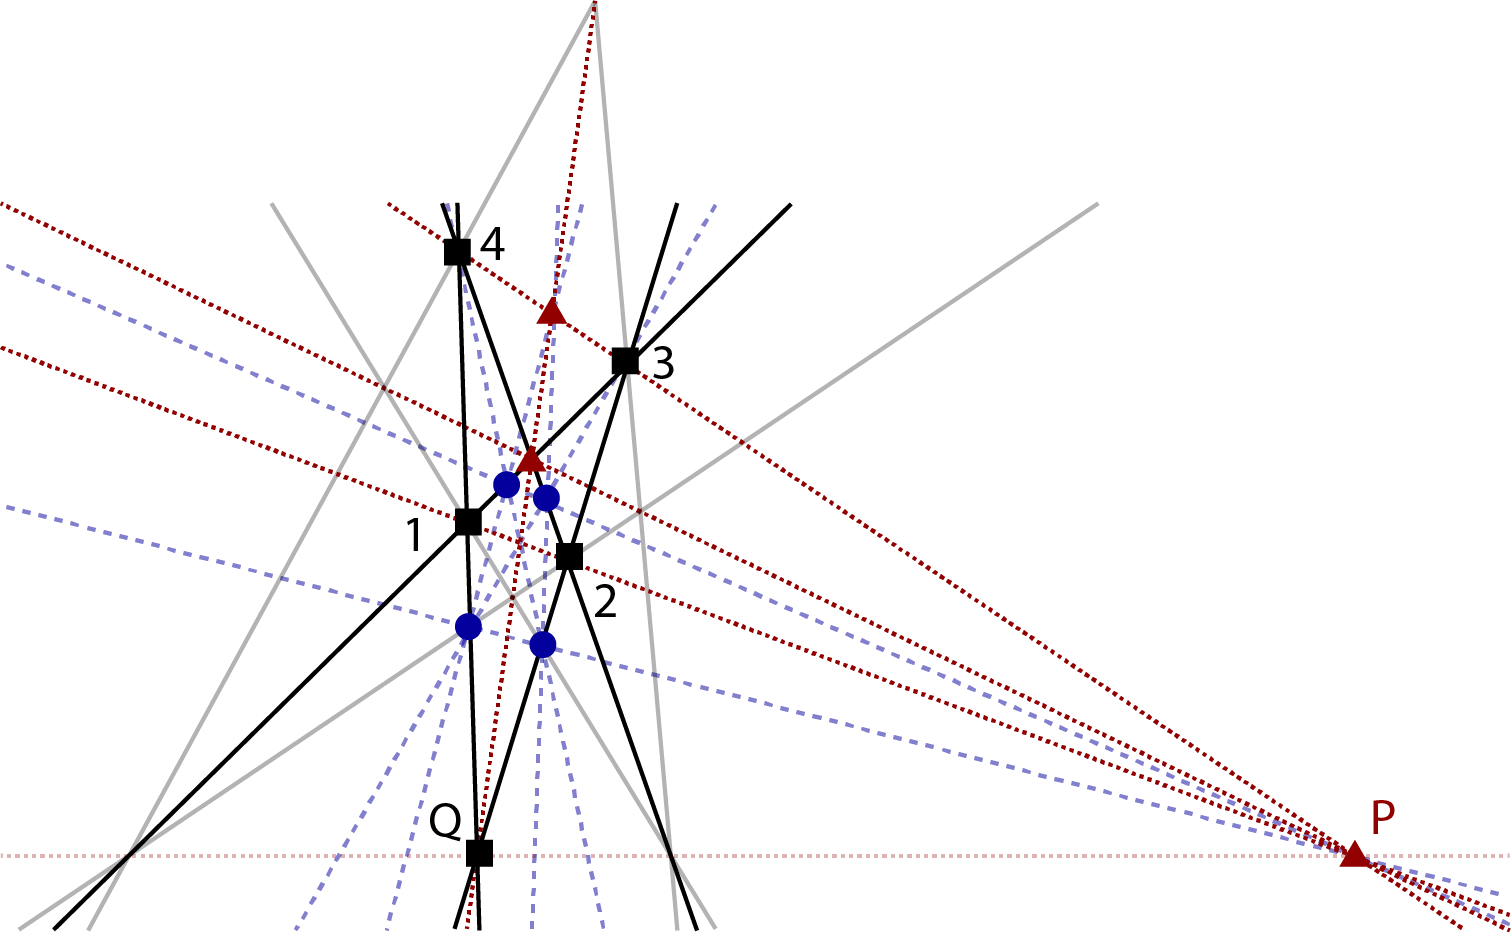
\includegraphics[width=0.35\textwidth]{Bilder/13_neu.png}
\caption{Weitere harmonische Grundfiguren in einer bereits vorhandenen}
\label{fig:13Neu}
\end{wrapfigure}

Zur Erklärung hier unsere Grundfigur mit anderen hervorgehobenen Linien. Aus der von uns konstruierten Grundfigur können wir nicht nur ein Viereck und ein Vierseit erkennen, sondern gleich mehrere, die wir so nicht vorgesehen hatten. Folglich lässt sich von zwei harmonischen Punkte-/Geradenpaaren eines als Nebenecke/-seite auffassen.

Auch lässt sich daraus erkennen, dass jedes einzelne Konstrukt innerhalb unserer Konfiguration die geometrischen Bedingungen der harmonischen Lage erfüllt.

Zusammengefasst ist

\begin{itemize}
\item[] jeder Schein eines harmonischen Punktewurfes ein harmonischer Geradenwurf
\item[] jeder Schnitt eines harmonischen Geradenwurfs ein harmonischer Punktewurf
\end{itemize}

Damit kommen wir zur Schlussfolgerung, dass die harmonische Lage eine projektve Invariante ist.

\glqq Man kann also schneiden und verbinden, soviel man will - einmal harmonisch heißt immer harmonisch.~\citep[s.~][S.~49]{projektiveGeometrie}\grqq

\newpage
\subsection{Erweiterung auf einen unendlich entfernten Punkt}

Unser bisher erlerntes Wissen können wir nun praktisch in die Tat umsetzen. Dabei lehnen wir uns an ein zeichnerisches Beispiel an, das den meisten aus der Schule bekannt vorkommen wird:

Wollen wir eine realistische Darstellung eines Gegenstandes auf Papier bannen, so beginnen wir als erstes damit, dass wir die Umgebung mit einer Horizontlinie definieren. Auf dieser Linie wählen wir mindestens einen Punkt aus, zu dem sich unser Gegenstand hin \glqq flüchtet\grqq . Dieser wurde als sogenannter \glqq Fluchtpunkt\grqq bezeichnet. Bezogen auf unser Thema ist dieser Punkt einer der Punkte, die wir zur Konstruktion der harmonischen Lage benötigen. Zur Konstruktion eines Gegenstandes (wählen wir dazu der Einfachheit eine quadratische Fläche) benötigen wir nur noch vier Geraden: zwei davon schneiden unseren Fluchtpunkt, während die anderen beiden, nach unserer Abbildung, parallel zum Horizont verlaufen. Die somit entstandene eingeschlossene Fläche ist unser Quadrat auf der projektiven Ebene.

\begin{figure}[htbp]
\centering
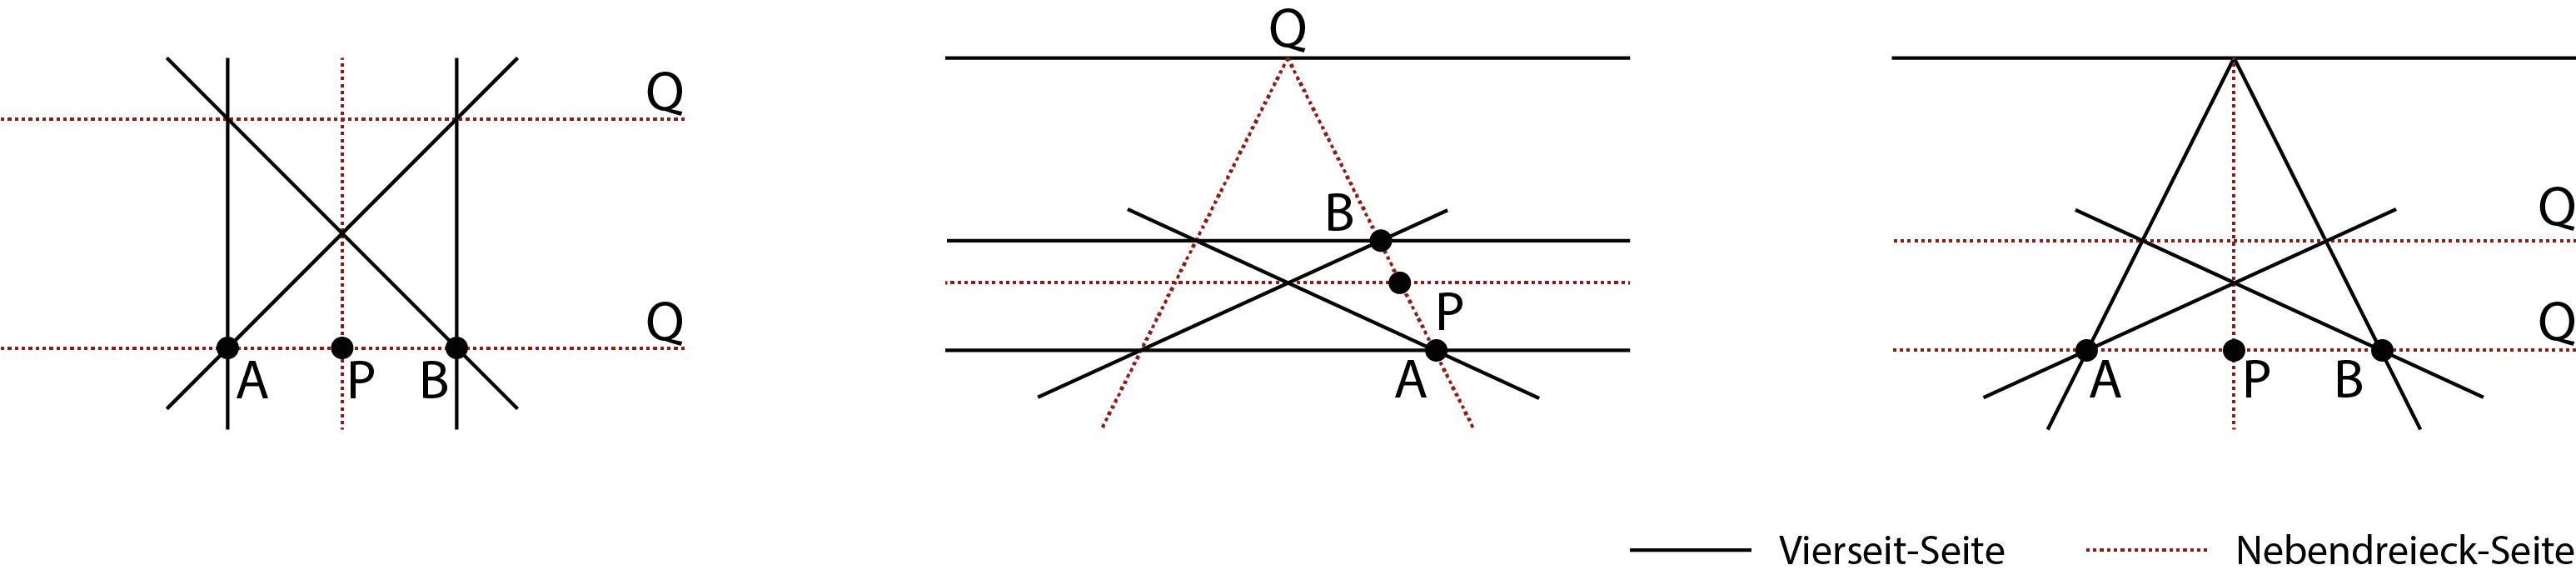
\includegraphics[width=\textwidth]{Bilder/inftyPoint.png}
\caption{Ist der Punkt Q ein unendlicher Fernpunkt, so trennt P die Strecke $\overline{A B}$ in der Mitte}
\label{fig:inftyPoint}
\end{figure}

Mit dieser Ausgangssituation können wir die harmonische Lage auf unser Quadrat anwenden. Dabei gehen wir genau so wie in unserem ersten Beispiel aus demselben Kapitel vor und erhalten eine harmonische Figur. Dabei lässt sich erkennen, dass die entstandene horizontale Gerade unser Quadrat in zwei Flächen teilt. Würden wir diese Situation senkrecht von oben betrachten würden wir erkennen, dass diese Gerade unser Quadrat genau in der Mitte teilt. Dabei handelt es sich nicht um einen Sonderfall. Jeder Punkt $P$, dessen Partner $Q$ ein Fernpunkt ist, teilt die Strecke $\overline{A B}$ immer genau in der Mitte.
\newline
Die Begründung ist einfach: Da die Konstruktion des vierten harmonischen Punktes, wie wir in der harmonischen 13er Konfiguration gesehen haben, nicht von der Wahl des jeweiligen Vierseits abhängt, können wir es uns einfach machen: wir wählen uns ein symmetrisches Vierseit, dessen einen Nebenseite die Symmetrie-Achse ist. Die dritte Nebenseite ist dann parallel zur zweiten \citep[vgl.~][S.~50]{projektiveGeometrie}.

Dabei taucht dieser Sachverhalt häufig in perspektivischen Abbildungen auf: Immer dann wenn wir eine Fläche in der Hälfte aufteilen, taucht die harmonische Lage auf, z.B.~ bei der Konstruktion eines Schachbretts. Dabei entsteht sogar, in Bezug zum Fluchtpunkt, eine Folge von harmonischen Punkten. Genaueres dazu wird in Kapitel \ref{sec:harmMittel} aufgegriffen.

\newpage
\section{Harmonische Lage rechnerisch}
Um nicht nur geometrisch und zeichnerisch auf die harmonische Lage von Punkten und Geraden schließen zu können, sondern auch mit Koordinaten arbeiten zu können, wird im folgenden das sogenannte Doppelverhältnis eingeführt. Anders Da aber das Doppelverhältnis per Definition ein Verhältnis ist, das aus zwei Teilverhältnissen besteht, wird vorab auf die Definition von Teilverhältnissen eingegangen.

\subsection{Teilverhältnisse}
\label{subsec:teilverh}
Sehen wir uns aber zuvor uns drei Punkte $A$, $B$ und $C$ auf einer Geraden $g$ an. Egal wie wir dieses drei Punkte auf dieser Geraden anordnen, es wird immer ein Punkt die Strecke zwischen seinen beiden Nachbarn in zwei kleinere Teilstrecken aufteilen. Dabei wird das Verhältnis dieser zwei Teilstrecken im allgemeinen definiert als

\[TV(A B C) = \overline{A C} : \overline{B C}\]

Wir sprechen hier vom sogenannten Teilverhältnis $TV$. Dabei soll $\overline{A B}$ als gerichteter Abstand zwischen $A$ und $B$ verstanden werden. D.h., $\overline{A B}$ und $\overline{B A}$ haben unterschiedliche Vorzeichen. Es gilt: 

\[\overline{A B} = -\overline{B A}\]

Man sagt auch, $C$ teilt das Punktepaar $(A , B)$ (bzw. die Strecke $\overline{A B}$) in diesem Verhältnis \citep[S.~76]{projektiveGeometrie}

Im Wesentlich haben wir, wenn wir vom Teilverhältnis sprechen, zwei unterschiedliche Betrachtungsweisen:
\begin{enumerate}
\item Befindet sich der Punkt $C$ zwischen den Punkten $A$ und $B$ (bzw. liegt auf $\overline{A B}$), so ist das Teilverhältnis negativ. Wir sagen: $C$ teilt das Punktepaar $(A , B)$ \glqq von innen\grqq .
\item Befindet sich der Punkt $C$ außerhalb den Punkten $A$ und $B$ (bzw. liegt auf $\overline{A B}$), so ist das Teilverhältnis positiv. Wir sagen: $C$ teilt das Punktepaar $(A , B)$ \glqq von außen\grqq .
\end{enumerate}

Wenn wir nun $C$ die gesamte Gerade durchlaufen lassen und beobachten den Wert $TV$, so können wir feststellen, dass der Wert von $TV$ stets monoton fallend ist. Wenn allerdings der Punkt $C$ auf $B$ fällt, so hat $TV$ den linksseitigen Grenzwert $-\infty$ und den rechtsseitigen Grenzwert $+\infty$.
\newpage
\begin{center}
\begin{scriptsize}
\begin{tabular}[htbp]{l|c|c|c|c|c|c|c|c}
$C$: & Fernp.~ & vor $A$ &  $A$ & zwi.~ $A$, $B$ & [Mitte] & $B$ & nach $B$ & Fernp.\\
\hline
$TV t$ & $t = 1 - o$ & $0 < t < 1$ & $t = 0$ & $t < 0$ & [$t = -1/2$] & $t = \pm\infty$ & $t > 1$ & $t = 1 + o$\\
\end{tabular}
\end{scriptsize}
\end{center}

\begin{figure}[htbp]
\centering
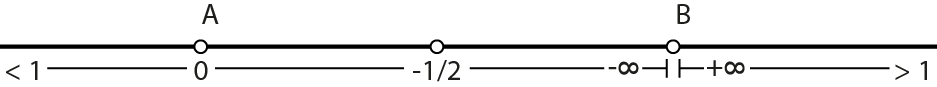
\includegraphics[width=\textwidth]{Bilder/tv_strahl.png}
\end{figure}

Da wir nun wissen, was man unter Teilverhältnissen versteht, können wir nun das Doppelverhältnis einführen:

\subsection{Das Doppelverhältnis}

Wie schon oben erwähnt ist das Doppelverhältnis das Verhältnis von zwei Teilverhältnissen von vier Punkten. Genauer gesagt, ist das Doppelverhältnis $DV$ von vier Punkten $A, B, C, D$, die auf einer Geraden $g$ liegen, definiert als das Verhältnis von $TV(A B C)$ und $TV(A B D)$:

\[DV(A B C D) = TV(A B C) : TV(A B D) = \dfrac{\overline{A C}}{\overline{B C}} : \dfrac{\overline{A D}}{\overline{B D}}\]

Anhand dieser Formel kann man erkennen, dass das Vorzeichen des Doppelverhältnisses
\begin{itemize}
\item negativ ist, wenn sich die Punktepaare $(A, B)$ und $(C, D)$ trennen. Dabei wird das Paar $(A, B)$ von $C$ und $D$ einmal innen und einmal von außen geteilt. Wir erhalten in den jeweiligen Teilverhältnissen zwei unterschiedliche Vorzeichen.
\item positiv ist, wenn sich die Punktepaare $(A, B)$ und $(C, D)$ nicht trennen. Beide Teilverhältnisse sind dann entweder nur positiv oder nur negativ.
\end{itemize}

Des Weiteren weist \citep{projektiveGeometrie} auf folgende Merkmale des Doppelverhältnisses hin:

Wenn $A = B$ oder $C = D$ ist und sonst keine Punkte zusammenfallen, dann ist das $DV = 1$.

Wenn $A = C$ oder $B = D$ ist und sonst keine Punkte zusammenfallen, dann ist das $DV = 0$.

Wenn $A = D$ oder $B = C$ ist und sonst keine Punkte zusammenfallen, dann ist das $DV = \pm\infty$.

Zusätzlich weist obige Formel ein paar interessante Eigenschaften auf, wenn Punkte in dieser Gleichung vertauscht werden \citep[vgl.][S.~77]{projektiveGeometrie}. Das Doppelverhältnis ändert sich nicht, wenn

\begin{enumerate}[label={\alph*)}] 
\item die Punkte innerhalb des 1. und zugleich des 2. Paares vertauscht werden,
\item das 1. mit dem 2. Paar vertauscht wird, und
\item sowohl die Paare als auch die Punkte innerhalb beider Paare vertauscht werden; also a) und b) zugleich.
\end{enumerate}

Somit gilt:

\[DV(A B C D) = DV(C D A B) = DV(B A D C) = DV(D C B A)\]

Damit ergeben sich auch aus den 24 Kombinationsmöglichkeiten von $A, B, C$ und $D$ folgende sechs verschiedene Zahlwerte \citep[s.][S.~77f]{projektiveGeometrie}:

\[z, ~~~~\dfrac{1}{z}, ~~~~1-z, ~~~~\dfrac{1}{1-z}, ~~~~\dfrac{z}{z-1}, ~~~~\dfrac{z-1}{z}\]

Hierbei ist $z = DV(A B C D)$.

\subsection{Harmonische Lage und Doppelverhältnis}

\begin{wrapfigure}{r}{0.4\textwidth}
\hspace{-0.025\textwidth}
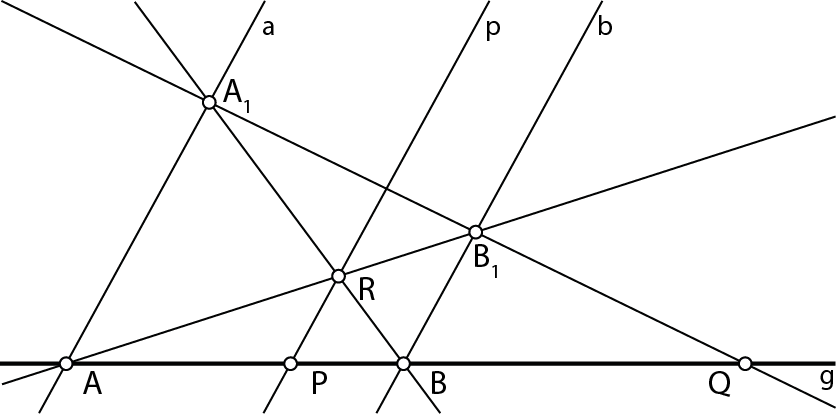
\includegraphics[width=0.45\textwidth]{Bilder/doppelverhaeltnis.png}
\caption{Harmonische Lage mit den parallelen Geraden $a$, $b$ und $p$}
\label{fig:harmonDoppel}
\end{wrapfigure}

Da wir jetzt die wichtigsten Eigenschaften des Doppelverhältnisses kennen, stellt sich uns nun die Frage, wie wir den Bogen zur harmonischen Lage schlagen. Betrachten wir die erste geometrische Konstruktion im Kapitel \ref{subsec:dieHarmonischeLage} dieser Arbeit nochmal an. Wir haben gesehen, dass wir zu jedem Punktepaar $(A, B)$ und einem Punkt $D$ einen weiteren Punkt $C$ bestimmen konnten, wobei die Punkte $A$, $B$ und $D$ festlagen. Wählen wir jetzt nur das Punktepaar $(A, B)$ fest und wählen irgendwo auf $g$ einen beliebigen Punkt $D$, so können wir auch sagen, dass es zu jedem $D$ genau ein Punkt $C$ gibt, sodass die Punkte $A, B, C, D$ in harmonischer Lage stehen bzw.~sich harmonisch teilen.

Betrachten wir nun die zwei Teilverhältnisse $TV(A B C)$ und $TV(A B D)$, so müssen wir feststellen, dass egal wie wir $D$ wählen, $TV(A B C) = -TV(A B D)$.

\citep{projektiveGeometrie} beweist diesen Sachverhalt mithilfe des Strahlensatzes. Dabei stellt sich der Autor die Frage, ob es zu einem gegebenen Punktepaar $(A, B)$ zwei Punkte $P$ und $Q$ gibt, die dieses Punktepaar im gleichen Verhältnis teilen, wobei $(A,  B)$ einmal von innen und einmal von außen geteilt werden, sodass

\[TV(A B P) = -TV(A B Q)\]

gelten müsste (vgl.~S.~52f). Dabei wird von folgender Ausgangssituation ausgegangen: Auf einer Geraden $g$ befinden sich zwei beliebige Punkte $A$ und $B$ und ein weiterer Punkt $P$. Es soll ein Punkt $Q$ konstruiert werden, sodass 

\begin{equation*}
\begin{split}
TV(A B P) = -TV(A B Q) \\
\Longleftrightarrow ~~~~~\overline{A Q} : \overline{B Q} = -\overline{A P} : \overline{B P}~~
\end{split}
\end{equation*}

Für einen einfacheren Umgang und besser mit Verhältnissen rechnen zu können, wurde eine Ausgangssituation mit zueinander parallelen Geraden gewählt, um Strahlensätze anwenden zu können (Abb.~\ref{fig:harmonDoppel}). Mithilfe der Strahlensatzgesetze können wir anhand von $A, B$ und $P$, einen Punkt $Q$ konstruieren:

\begin{equation*}
\begin{split}
  \overline{A P} : \overline{B P}~ \\
=~~~\overline{A R} : \overline{B_1 R}  \\
=~~\overline{A A_1} : \overline{B_1 B}  \\
=~~~\overline{Q A} : \overline{Q B}~
\end{split}
\end{equation*}

Daraus lässt sich schließen, dass die zwei Punkte $A$ und $B$ von $P$ und $Q$ von innen und von außen gleich getrennt werden, wenn die Punktepaare in harmonischer Lage sind. Zusätzlich ergibt sich aus der Gleichung, dass zwei Punktepaare $(A, B)$ und $(P, Q)$ genau dann in harmonischer Lage sind, wenn das Doppelverhältnis -1 beträgt:

\begin{equation*}
\begin{split}
TV(A B P) = -TV(A B Q) \Longleftrightarrow TV(A B P) : TV(A B Q) = -1 \\ \Longleftrightarrow ~~~~~~~~~~~~~~DV(A B P Q) = -1
\end{split}
\end{equation*}

\subsection{Das Doppelverhältnis von vier Geraden}

Bisher haben wir nur das Doppelverhältnis von Punkten betrachtet, die sich alle auf ein und derselben Gerade befanden. Jedoch kann man die Definition des Doppelverhältnisses zusätzlich auf vier Geraden erweitern. Wie bei dem Doppelverhältnis von vier Punkten, bei der die Ausgangssituation darauf festgelegt war, dass sich diese Punkte auf einer Gemeinsamen Geraden befinden, gilt für das Doppelverhältnis vierer Geraden $a, b, c$ und $d$, dass sich diese in einem gemeinsamen Punkt $P$ schneiden (Abb. \ref{fig:vierGeraden}). Dabei wird $P$ auch Projektionszentrum genannt.

Schneiden wir nun diese vier Strahlen mit einer beliebigen Geraden $g$, wobei diese nicht durch den Punkt $P$ gehen darf, so erhalten wir vier Schnittpunkte $A, B, C$ und $D$. Weiter fällen wir die Lote von $A$ und $C$ auf $b$ und $d$ mit den Schnittpunkten $Q_1, Q_2$ und $R_1, R_2$. Es entstehen rechtwinklige Dreiecke. Mit dem Strahlensatz sowie dem Sinus (insbesondere dem Verhältnis von Gegenkathete und Hypothenuse) lässt sich jetzt unsere vorher bekannte Definition des Doppelverhältnisses auf folgende Formel umändern \citep[s.~][S.~80]{projektiveGeometrie}: 

\begin{equation*}
\begin{split}
DV(A B C D)~=~~~~~~~~~~~~~\dfrac{\overline{A C}}{\overline{B C}} : \dfrac{\overline{A D}}{\overline{B D}}~~~~~~~~~~~~\\
=~~~~~~~~~~~~\dfrac{\overline{A Q_1}}{\overline{B Q_2}} : \dfrac{\overline{A R_1}}{\overline{B R_2}}~~~~~~~~~~~\\
=~\dfrac{\overline{A P} * sin(ab)}{\overline{B P} * sin(cb)} : \dfrac{\overline{A P} * sin(ad)}{\overline{B P} * sin(bd)} \\
=~~~~~~~~\dfrac{sin(ac)}{sin(bc)} : \dfrac{sin(ad)}{sin(bd)}~~~~~~~~
\end{split}
\end{equation*}

Somit können wir nicht nur das Doppelverhältnis nur anhand von Punkten auf einer Geraden $g$ bestimmen, sondern auch durch die Geraden der Punkte, die sich auf einem von $g$ außerhalb liegenden Punkt schneiden. Das bedeutet auch, dass egal was für eine Gerade wir nehmen, die die Geraden $a, b, c$ und $d$ schneiden und nicht durch $P$ gehen, das Doppelverhältnis das Gleiche ist. Damit ist auch das Doppelverhältnis eine projektive Invariante. Mithin trifft dies auch auf die harmonische Lage zu, was wir aber auch durch Invarianzen in Kapitel \ref{subsec:harmonischeKonfiguration} gesehen haben.

\begin{figure}[htbp] 
\centering
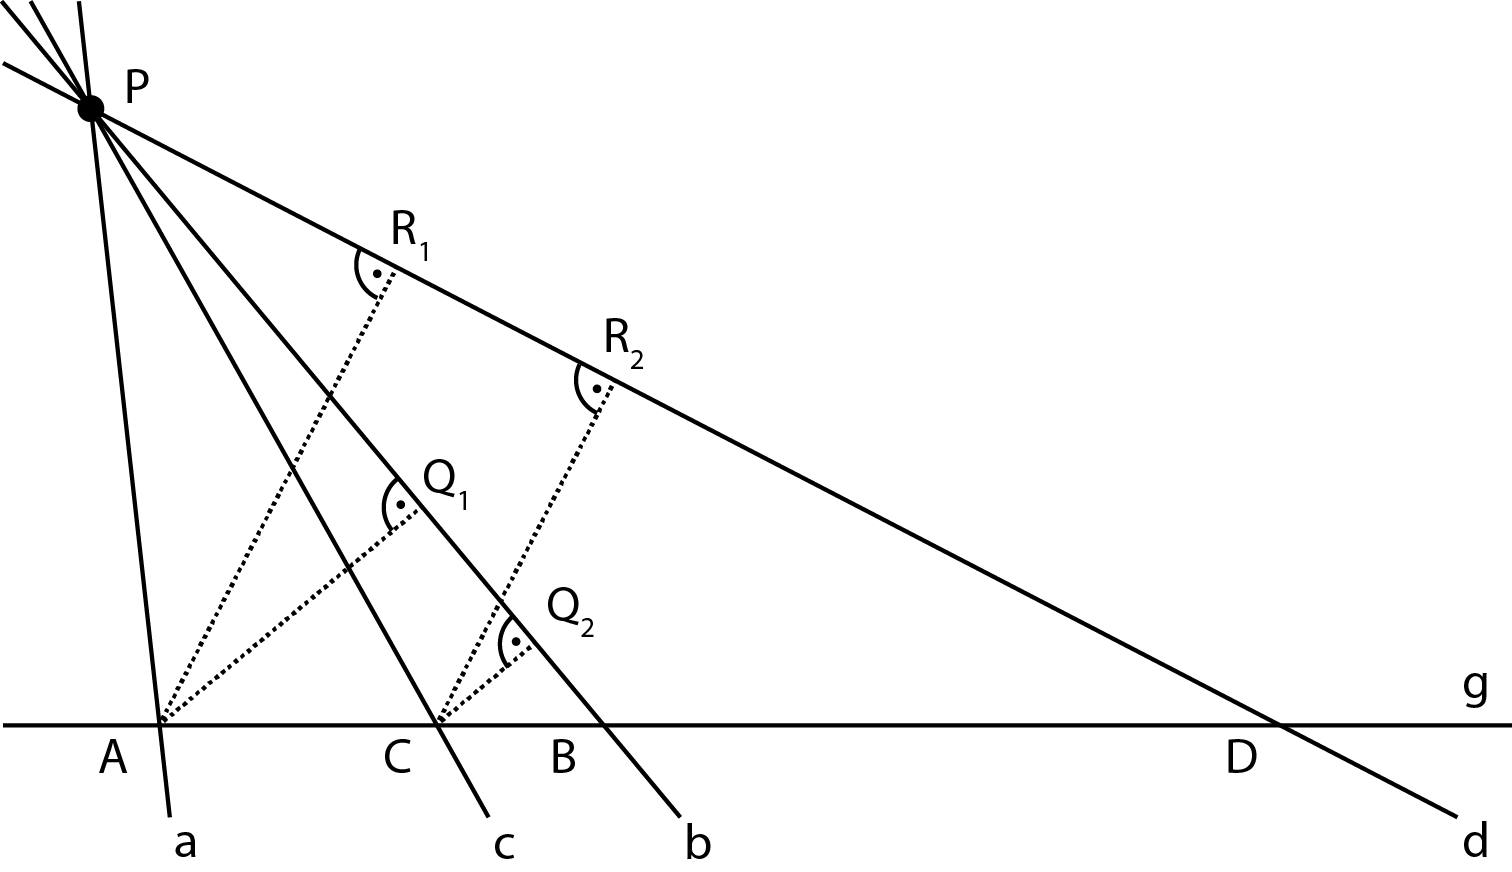
\includegraphics[width=0.7\textwidth]{Bilder/vierGeraden.png}
\caption{Ermittlung der harmonischen Lage durch vier Geraden}
\label{fig:vierGeraden}
\end{figure}

\newpage
\section{Harmonisches Mittel und harmonische Folge}
\label{sec:harmMittel}

Die Bezeichnung \glqq harmonisch\grqq taucht nicht nur in der projektiven Geometrie auf. Allerdings können wir diese mit diesem Themengebiet in Verbindung bringen:

\subsection{Harmonisches Mittel}

Der Begriff des arithmetischen Mittels ist ein sehr geläufiger Begriff. Dabei handelt es sich beim arithmetischen Mittel um den Mittelwert, der die Summe der betrachteten Zahlen durch dessen Anzahl geteilt wird.

\[x_a = \dfrac{1}{n} \sum_{i=0}^n x_i = \dfrac{x_1 + x_2 + \dots + x_{n-1} + x_n}{n}\]

Ebenso bekannt in der Mathematik ist auch der sogenannte harmonische Mittelwert. Das harmonische Mittel ist das Gegenstück zum arithmetischen Mittel, bzw.~ der Kehrwert des harmonischen Mittels das arithmetische Mittel der Kehrwerte:

\[ \dfrac{1}{x_h} = \dfrac{1}{n} \sum_{i=0}^n \dfrac{1}{x_i} = \dfrac{\dfrac{1}{x_1} + \dfrac{1}{x_2} + \dots + \dfrac{1}{x_{n-1}} + \dfrac{1}{x_n}}{n}\]

Somit ist das harmonische Mittel

\[ x_h = \dfrac{n}{\dfrac{1}{x_1} + \dfrac{1}{x_2} + \dots + \dfrac{1}{x_{n-1}} + \dfrac{1}{x_n}}.\]

Der Zusammenhang zwischen der harmonischen Lage und dem harmonischen Mittel lässt sich einfach miteinander verbinden. Denn vom Kapitel über das Doppelverhältnis wissen wir, dass sich zwei Punktepaare $(A, B)$ und $(C, D)$ sich harmonisch trennen, wenn sie sich innen und außen gleich teilen:

\[|TV(A B C)| = |TV(A B D)|\]

Definieren wir $b = |\overline{A B}|$, $c = |\overline{A C}|$ und $d = |\overline{A D}|$.Durch umformen ergibt sich

\begin{equation*}
\begin{split}
|TV(A B C)|~=~|TV(A B D)| ~\\
\Longleftrightarrow ~~~~~~~~~\dfrac{c}{b-c}~=~\dfrac{d}{d-b}~~~~~~~~~~\\
\Longleftrightarrow ~~~~~~~cd-cb~=~db-cd~~~~~~~~\\
\Longleftrightarrow ~~~~~~~~~~~~2 cd~=~d (c+b)~~~~~~~\\
\Longleftrightarrow ~~~~~~~~~\dfrac{2cd}{c+d}~=~b,~~~~~~~~~~~~~~~\\
\end{split}
\end{equation*}

woraus wir erkennen können, dass $b$ das harmonische Mittel von $c$ und $d$ ist. Indem wir einen Punkt auf unserer Geraden festlegen und mithilfe zweier Abstände zu gegebenem Punkt zwei weitere Punkte bestimmen, können wir mit dem harmonischen Mittelwert den vierten Punkt berechnen. Legen wir Punkt $A$ als Nullpunkt fest, können wir die Abstände als Koordinaten definieren.

Ein Sonderfall bei der Auswahl unseres Punktes tritt dann auf, wenn wir den vierten Punkt so wählen, dass dieser ein Fernpunkt ist. Ist dies der Fall tritt hier sogar das arithmetische Mittel auf. Dies liegt daran, dass wir zwar immer noch das harmonische Mittel vorliegen haben, aber unser gewählter Punkt im Bezug zum Fernpunkt $\infty$ steht.

Diese Sachverhalte sind gut in den sogenannten Möbius'sche Netze nachzuvollziehen (Abb.~\ref{sec:harmMittel}). Indem wir ein solches Netz aufbauen, können wir unendlich viele 4. harmonische Punkte hinzu konstruieren: in die eine Richtung verdichtend, in die andere ausdehnend. Definieren wir unsere 3 Grundpunkte als 0, 1 und $\infty$, lassen sich sehr schöne Zahlenfolgen Konstruieren. Dabei fällt auf, wenn wir von einer ausgesuchten Zahl $n$ unserer Konstruktion seine beiden Nachbarn $n-1$ und $n+1$ betrachten, dass n das harmonische Mittel von $n-1$ und $n+1$ ist. Somit ist das harmonische Mittel Bestandteil harmonischer Lage-Beziehungen von Punkten.



\begin{figure} [htbp]
\subfigure[Harmonisches Mittel]{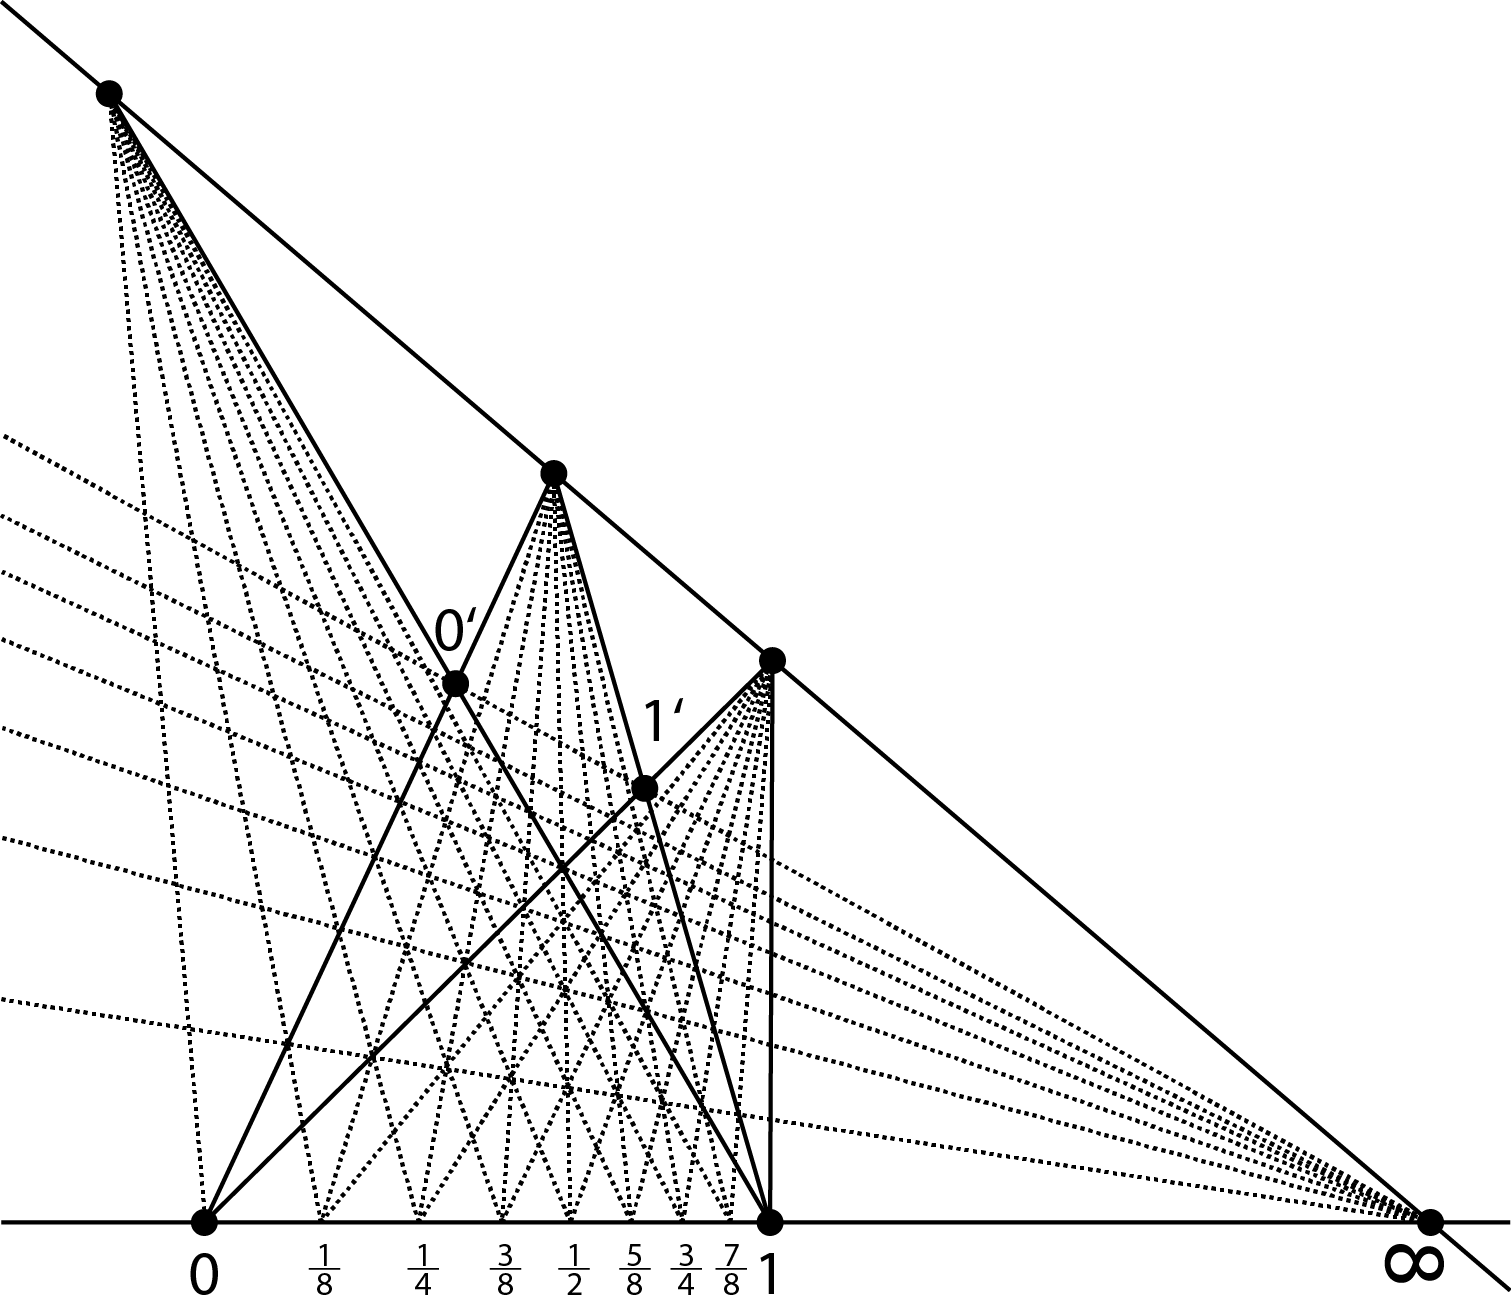
\includegraphics[width=0.4\textwidth]{Bilder/harmMittel.png}} \hfill
\subfigure[Harmonisches und arithmetisches Mittel]{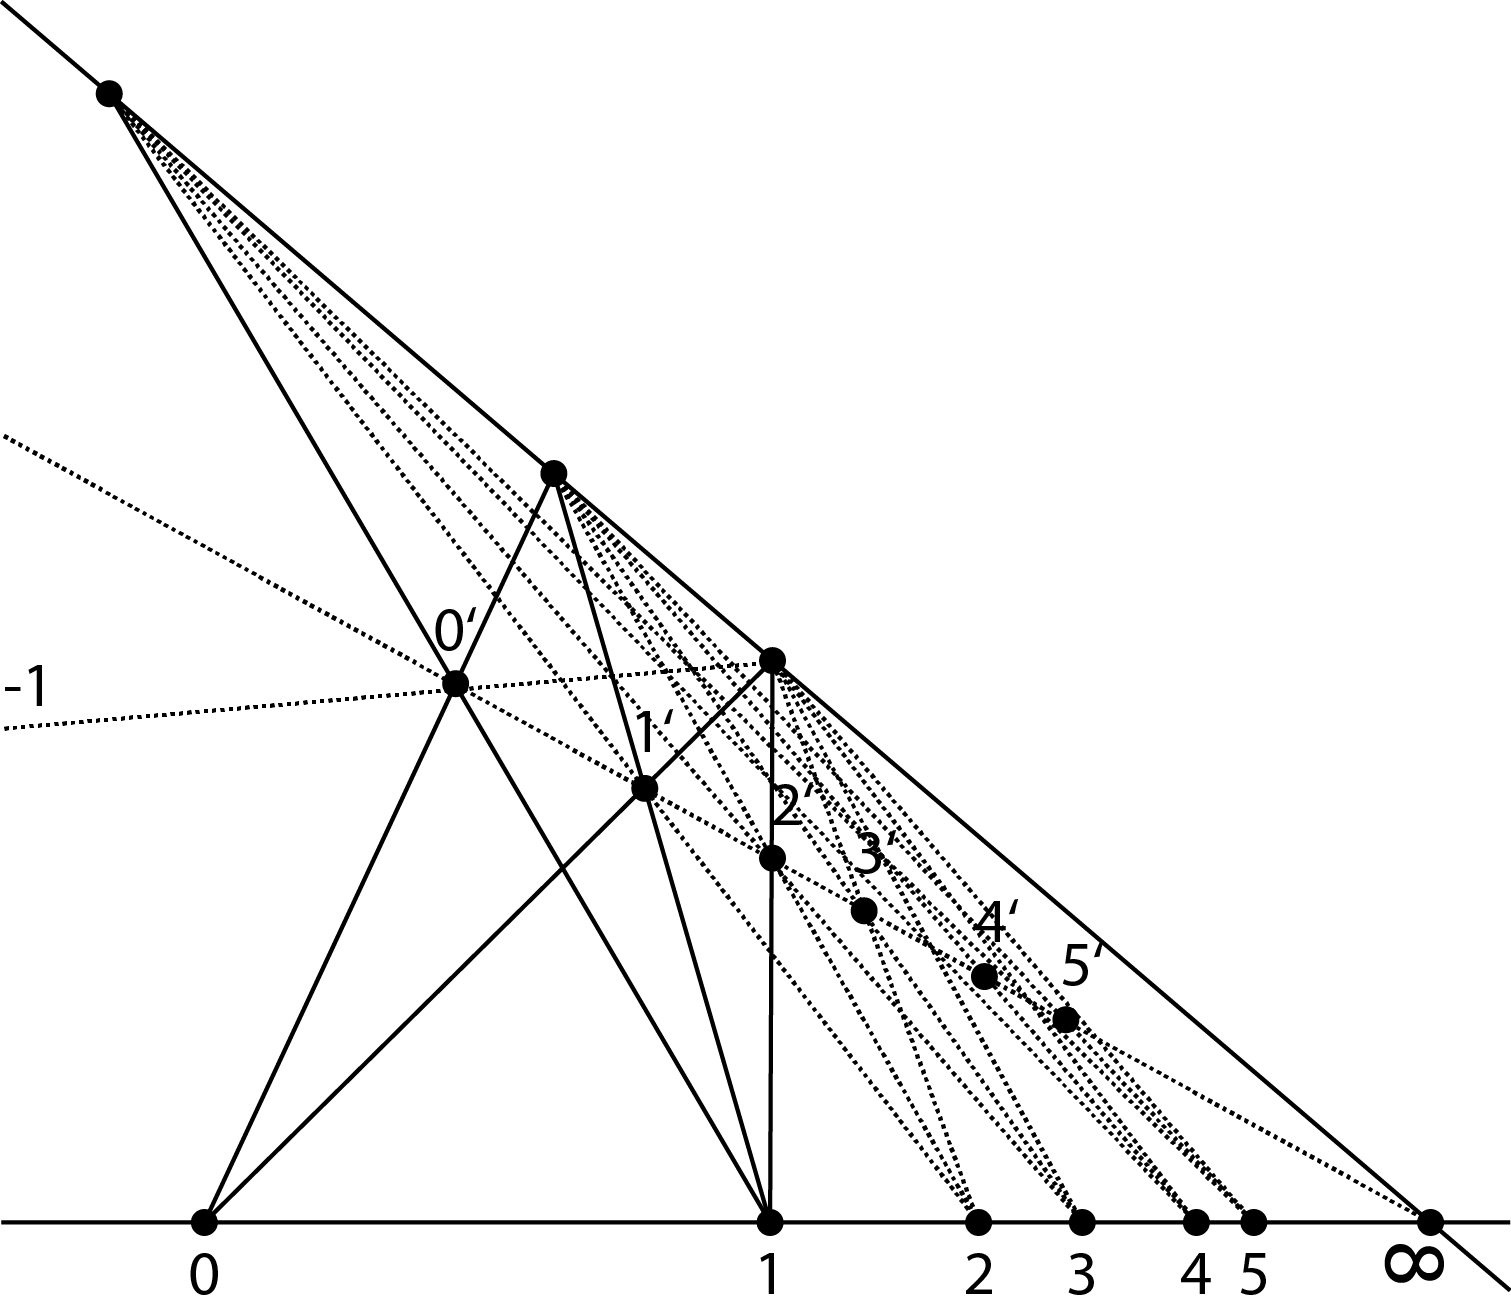
\includegraphics[width=0.4\textwidth]{Bilder/harmMittel2.png}}
\caption{Möbius'sche Netze in Verdichtung und Dehnung}
\end{figure} 

\newpage
\subsection{Harmonische Folge}
\label{subsec:harmFolge}

Auch bekannt im Bereich der Zahlenfolgen ist die harmonische Folge. Dabei ist jedes Glied dieser Folge der Kehrwert der positiven ganzen Zahlen und somit Kehrwert der Glieder einer arithmetischen Folge: 

\[ 1,~~~~~\dfrac{1}{2},~~~~~\dfrac{1}{3},~~~~~\dfrac{1}{4},~~~~~\dfrac{1}{5},~~~\dots\]

\[ a_n = \dfrac{1}{n} ~~~~~ n \geq 1\]

Des Weiteren ist jedes Glied der Folge (mit der Voraussetzung $n \geq 2$) das harmonische Mittel seiner beiden Nachbarglieder. Betrachten wir die harmonische Folge als Funktion, so konvergiert diese gegen 0:

\[ \lim_{x \to \infty} \dfrac{1}{n} = 0\]

Auch zu beachten bei der harmonischen Folge ist, wenn jedes Folgenglied mit einer Konstanten multipliziert wird, dass daraus wieder eine harmonische Folge entsteht.

Beziehen wir die harmonische Folge auf die harmonische Lage von Punkten: Zur Vereinfachung legen wir $A$ als Nullpunkt fest, damit wir anstelle von Abständen mit Koordinaten arbeiten können. Der Partner von $A$ sei der Punkt $B$, den wir mit 1 identifizieren. Legen wir nun einen Punkt $D$ fest, der Folgenglied einer arithmetischen Folge ist, so erhalten wir mithilfe des Kehrwertes den Punkt $C$. Dabei trennt $B$ die Punkte $C$ und $D$ im harmonischen Mittel. Wir können also für $D \geq 1$ immer das passende harmonische Folgenglied finden und erhalten somit zwischen 0 und 1 für alle Punkte von $C$ eine harmonische Folge. Dabei ist der Gegenpunkt von $C$ - der Punkt $D$ - das Folgenglied einer arithmetischen Folge. Wenn wir demnach eine Skala zeichnen, auf der wir die harmonische sowie die arithmetische Folge haben, und verbinden die Punkte der Skala mit einem beliebigen Punkt $P$ außerhalb davon, so erhalten wir einen Wurf harmonischer Geraden. Dabei treten folgende harmonische Punktepaar-Beziehungen für die harmonische Folge $\dfrac{1}{n}$ und die arithmetische Folge $n$ mit jeweils $n \geq 1$ auf:

\begin{itemize}
\item $\left(0, 1\right)$ und $\left(\dfrac{1}{n}, n\right)$ für $n \geq 1$,
\item $\left(n-1, n+1\right)$ und $\left(n, \infty\right)$ für $n \geq 2$, sowie
\item $\left(0, \dfrac{1}{n}\right)$ und $\left(\dfrac{1}{n+1}, \dfrac{1}{n-1}\right)$ für $n \geq 2$.
\end{itemize}

\begin{figure}[htbp]
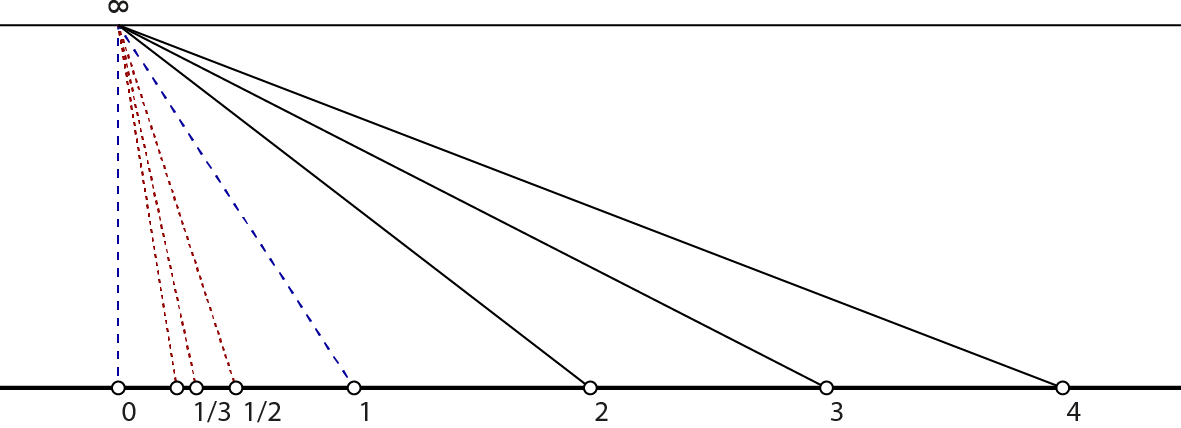
\includegraphics[width=\textwidth]{Bilder/folge.png}
\end{figure}

\newpage
\section{Harmonische Lage und Goldener Schnitt}

Bevor wir den theoretischen Teil beenden und uns der Praxis zuwenden können, fehlt uns noch ein einzelner Aspekt in der geometrischen und arithmetischen Mathematik, bei dem wir ebenfalls die harmonische Lage vorfinden: nämlich dem Phänomen des Goldenen Schnittes.

Der Goldene Schnitt tritt seit der Antike in  vielen Bereichen der Geometrie, Architektur, Musik, Kunst sowie der Philosophie auf aber er erscheint auch heutzutage in den Gebieten von Design und Technik. Dabei ist der Goldene Schnitt kein isoliertes Phänomen, sondern in vielen Fällen das erste und somit einfachste nichttriviale Beispiel im Rahmen weiterführender Verallgemeinerungen \citep[s.][S.~5]{goldenerSchnitt}.

Dabei ist der Goldene Schnitt ein Teilverhältnis (wir erinnern uns Kapitel \ref{subsec:teilverh}), welches in verschiedenen geometrischen und arithmetischen Situationen erscheint. Dieses Teilverhältnis ist definiert als das Verhältnis zweier Streckenabschnitte zueinander, die sich genauso verhalten wie die der längere Abschnitt zur gesamten Strecke:

\[\dfrac{b}{a} = \dfrac{a}{c}\]

Setzen wir $c = 1$, können wir das Verhältnis des Goldenen Schnittes bestimmen:

\[\dfrac{1-x}{x} = x\]

Durch umformen erhalten wir eine quadratische Gleichung

\[x^2 + x - 1 = 0\].

Diese hat die beiden Lösungen

\[x_1 = \dfrac{-1 + \sqrt{5}}{2} \approx 0,618~~ \]

und

\[ x_2 = \dfrac{-1 - \sqrt{5}}{2} \approx -1,618 \].

Da $x$ positiv sein muss, muss $x_1$ unsere Lösung sein. Somit ist die Zahl des Goldenen Schnittes $\dfrac{\sqrt{5}-1}{2}$. Der Kehrwert ist dann $\dfrac{\sqrt{5}+1}{2}$.

Da wir sowohl bei der harmonischen Lage als auch beim Goldenen Schnitt von von Teilverhältnissen sprechen, können wir diese zwei geometrischen Aspekte miteinander verbinden.

Nehmen wir dazu folgende Situation an: Auf einer Geraden befinden sich zwei Punkte $A$ und $B$, deren Strecke $\overline{A B}$ von einem weiteren Punkt $C$ im Goldenen Schnitt geteilt wird. Demnach ist das Teilverhältnis $TV(A B C) = \overline{A C} : \overline{B C}$ gleich dem Teilverhältnis $TV(C B A) = \overline{C A} : \overline{B A}$. Dies kann auch anhand der Vertauschungsregeln aus Kapitel \ref{subsec:teilverh} nachgeprüft werden:

Sei $TV(A B C) = z$, so ist

\begin{equation*}
\begin{split}
TV(A B C)~=~\overline{A C}~:~\overline{B C}\\
=~\dfrac{z}{1-z}~~~~~~\\
=TV(C B A).
\end{split}
\end{equation*}

Hier ist aber zu beachten, dass wir hier ungerichtete Abstände betrachten.

Indem wir nun mithilfe der harmonischen Lage weitere Punkte und Abstände bestimmen können, die zueinander im Goldenen Schnitt stehen, erhalten wir dadurch eine Folge von Abständen mit dem Teilverhältnis $\dfrac{\sqrt{5}-1}{2}$.

\newpage
\section{Harmonische Lage in der Gestaltung}

Nach so viel Theorie wollen wir uns den praktischen Bezug der harmonischen Lage genauer ansehen. Hierbei legen wir unser Augenmerk in Richtung Kunst und Design. Zum Einstieg für die harmonische Lage in der Kunst können wir unser Wissen aus den vorherigen Kapiteln nutzen, wobei wir für die harmonische Lage im Design noch einen kurzen Einstieg in den Goldenen Schnitt erfordert.

\subsection{Harmonie in der Malerei}

Vielen von uns ist der Begriff der Perspektive wahrscheinlich größtenteils mit fotorealistischen Gemälden und Bildern gekoppelt. Tatsächlich fand die Perspektive nach ihrer Wiederentdeckung im 15. Jahrhundert, wahrscheinlich um 1413 \citep[S.~27]{perspektive}, neben der Geometrie auch hauptsächlich in der Bildenden Kunst bzw.~ der Malerei Anwendung. Vor ihrer Entdeckung mussten sich die Maler an einem Kanon von Regeln halten, denen es erlaubte, einigermaßen räumliche Szenen darzustellen. Jedoch beruhten diese auf keinerlei wissenschaftlich gesicherten Einsichten.

\begin{wrapfigure}{r}{0.4\textwidth}
\centering
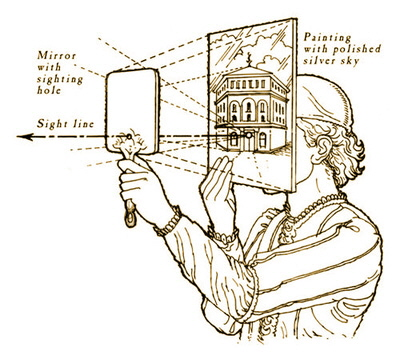
\includegraphics[width=0.4\textwidth]{Bilder/Brunelleschi-Zentralperspektive.jpg}
\caption{Das  Spiegelexperiment}%www.medien-gesellschaft.de/html/geschichte_des_sehens.html
\label{fig:brunnelli1}
\end{wrapfigure}

Fangen wir also ganz zu Beginn an: Die ersten Aufzeichnungen der Wiederentdeckung der Perspektive lassen sich in den Schriften vom Biographen Antonio Mannetti finden. Diese handeln allerdings nicht von Erkenntnissen, die Mannetti entdeckt hatte, sondern beschreiben die Arbeiten des Bildhauers und Architekten Filippo Brunelleschi. Dieser hatte in einem seiner ersten Experimente ein Miniaturenbild der Florentiner Taufkapelle, die von ihm so exakt wie möglich gezeichnet wurde. Zusätzlich legt er den Himmel mit poliertem Silber aus, um den realen Himmel darauf abbilden zu können. Doch benutzte er das Werk nicht zur Zurschaustellung, sondern für ein Experiment: Brunelleschi Bohrte in den Eingangsbereich der Taufkapelle ein Loch. Durch dieses Loch sollte ein Betrachter von der Rückseite des Bildes auf das Gebäude sehen. Dabei sollte der Betrachter an einer von Brunelleschi bestimmten stelle stehen. Der zweite Teil des Experimentes bestand darin, einen Spiegel zwischen Gebäude und Abbildung zu stellen, sodass die Sicht vom Spiegel verdeckt wurde. Allerdings sah der Betrachter nun die von Brunelleschi hergestellte Abbildung. Die illusionistische Wirkung musste überwältigend gewesen sein \citep[S.~28f]{perspektive}.

Interessant ist jedoch hier, dass Brunelleschi es geschafft hatte, die mathematische Theorie des Sehens von Euklid mit der Theorie der Zentralprojektion zu verbinden. Dabei befindet sich das Guckloch des Bildes genau im Projektionszentrum und Hauptfluchtpunkt des Bildes \citep[S.~30]{perspektive}.

Im Jahre 1435/36 veröffentlichte Leon Battista Alberti in seinen \textit{Drei Bücher über die Malerei} die theoretischen Grundlagen, die Filippo Brunelleschi verwendet hatte. Dabei beschrieb er den Horizont und den Fluchtpunkt. Aus Brunelleschis Experimenten erfuhr Alberti, dass parallel verlaufende Strecken auf einen Punkt hin konvergieren, der unendlich weit vom Betrachter weg scheint. Um aber ein Maß zwischen Bildfläche und Fluchtpunkt bestimmen zu können, um Distanzen auf der perspektivischen Zeichenfläche besser darzustellen, ging Alberti wie folgt vor:

Um ein anschauliches Maß zu finden betrachtete Alberti quadratische Fliesen auf dem Boden. Er legte fest, dass ein Mensch, oder genauer gesagt die Augenhöhe eines Menschen, durchschnittlich 3 \textit{braccia} (ital.~ für \glqq Arme\grqq) beträgt. Dabei entsprechen drei \textit{braccia} ungefähr 174cm. Mit dieser Angabe legte er die Horizontlinie fest. Den unteren Rand des Bildes unterteilte Alberti gleichmäßig in die Anzahl der Fliesen in der horizontalen. Dann wurde der Hauptfluchtpunkt festgelegt, der nach Alberti auf Augenhöhe liegen musste. Somit musste dieser Punkt auf der Horizontlinie liegen. Mit diesen Punkt verband Alberti die maßgebenden Punkten am unteren Bildrand, sodass mehrere Pyramiden entstanden. Damit wären schon mal die Parallelen Linien in die Tiefe geschaffen.

Bisher wurde immer die Pyramiden im Verhältnis $2 : 3$ geteilt, womit ein abgefälschtes Maß für Linien entstanden, die parallel zum Horizont liegen. Denn je nach dem sich der Betrachter von der Bildfläche entfernt, so mussten die Abstände zwischen diesen Parallelen der Abstand in einem natürlichen Maß kleiner werden. Alberti nahm sich dazu im Gegensatz zur bisherigen Vorgehensweise was anderes vor. Er konstruierte sich eine Seitenansicht des Geschehens, wo sich Bild, Kacheln und sogar der Betrachter der Szene befinden. Indem er wusste, mit welchem Abstand sich der Betrachter vom Bild weg befindet, konnte er den Augenpunkt exakt bestimmen. Die Strecke hinter der Bildfläche unterteilte Alberti wieder in der Anzahl der Fliesen. Diese Unterteilungspunkte verband er mit dem Augenpunkt. Dabei gaben die Schnittpunkte der Verbindungsstrecken mit der Bildfläche die Positionen der Parallelen im Bild an (Abb.~\ref{fig:braccia}, \citep[vgl.][S.~31ff]{perspektive}).

\begin{figure}[htbp] 
\centering
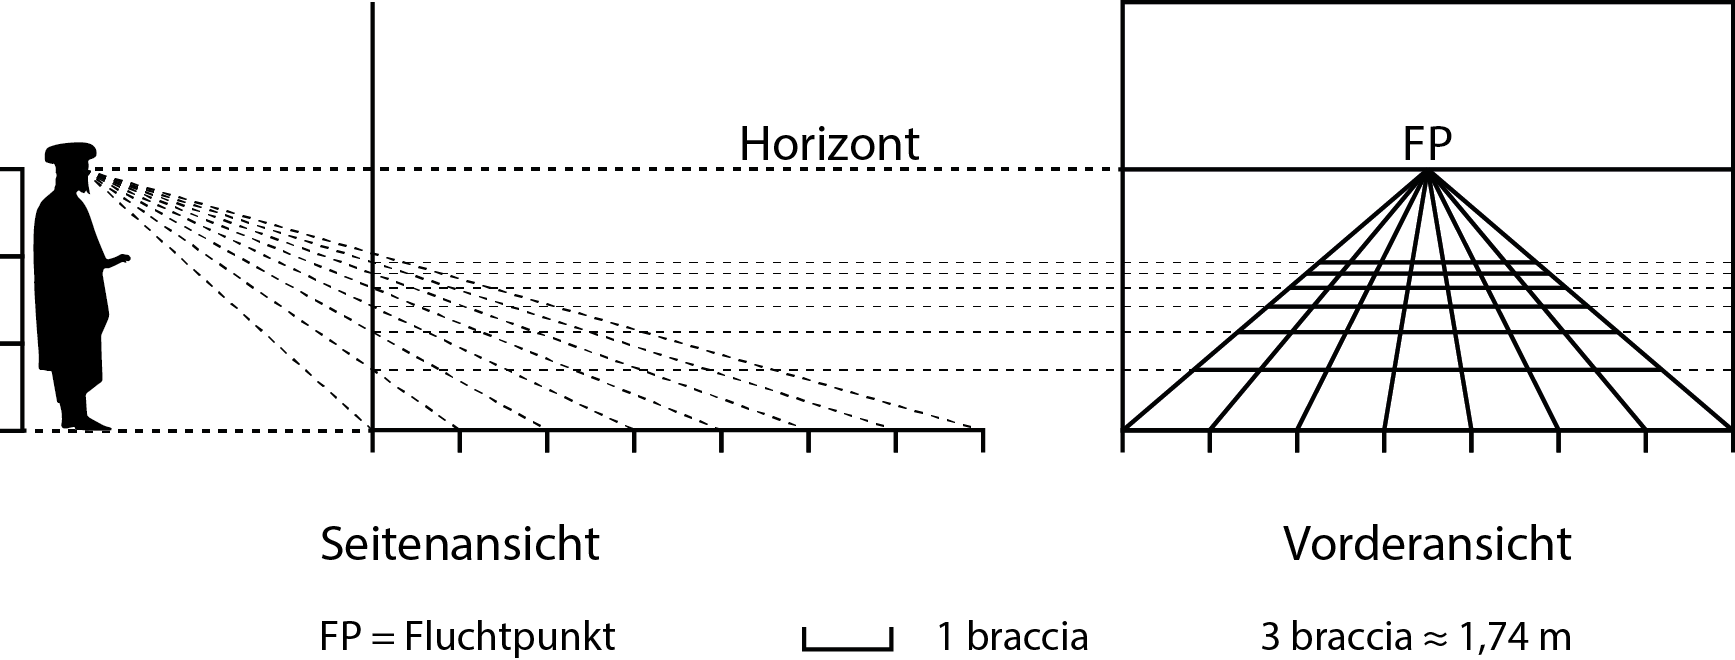
\includegraphics[width=\textwidth]{Bilder/braccia.png}
\caption{Zeichnerischer Weg zur Zentralperspektive nach Leon Battista Alberti}
\label{fig:braccia}
\end{figure}

Mit dieser sehr geschickt gewählten Methode war es ab sofort möglich, jegliche Gegenstände perspektivisch Korrekt darzustellen. Im Laufe der Jahre wurde Albertis perspektivische Konstruktion von Personen wie Albrecht Dürer und Leonardo DaVinci auf mehrere Fluchtpunkte ausgeklügelt und mathematisch begründet. Doch kann dies als Grundstein für die nachkommenden perspektivischen Werke in der Kunstgeschichte betrachtet werden. Dabei kann die Konstruktion solcher perspektivischen Raster nicht nur zum Bildrand parallele Flächen angewandt werden, sondern sie kann auch für vertikale und schräge Raster verwendet werden.

%TODO Beispielbilder

Tatsächlich sollte auch hier unser nun geschultes Auge erkennen, dass solche und andere perspektivischen Konstruktionen unserer Definition von harmonischen Punkten und Geraden entsprechen. Hier taucht sogar die Harmonische Lage mehrfach auf: Zum einen in der fertigen Konstruktion, zum anderen aber auch bei den Verbindungslinien zwischen der Skala und dem Augenpunkt (s.~ Kapitel \ref{subsec:harmFolge}).

Egal ob wir nur einen oder mehrere Fluchtpunkte in unserem Bild haben, alle auf diesen Punkt konvergierende Geraden stehen immer in harmonischer Lage zueinander. Indem wir ähnlich Alberti perspektivische Raster durch die Konstruktion harmonischer Punkte erhalten, ist die Harmonische Lage ein Maß für den menschlichen Sehsinn, den wir auch für Bilder, Gemälde o.ä.~verwenden können.

\newpage
\subsection{Harmonische Lage im Design}

\subsubsection{Satzspiegel}

\begin{wrapfigure}{r}{0.4\textwidth}
\hspace{-0.025\textwidth}
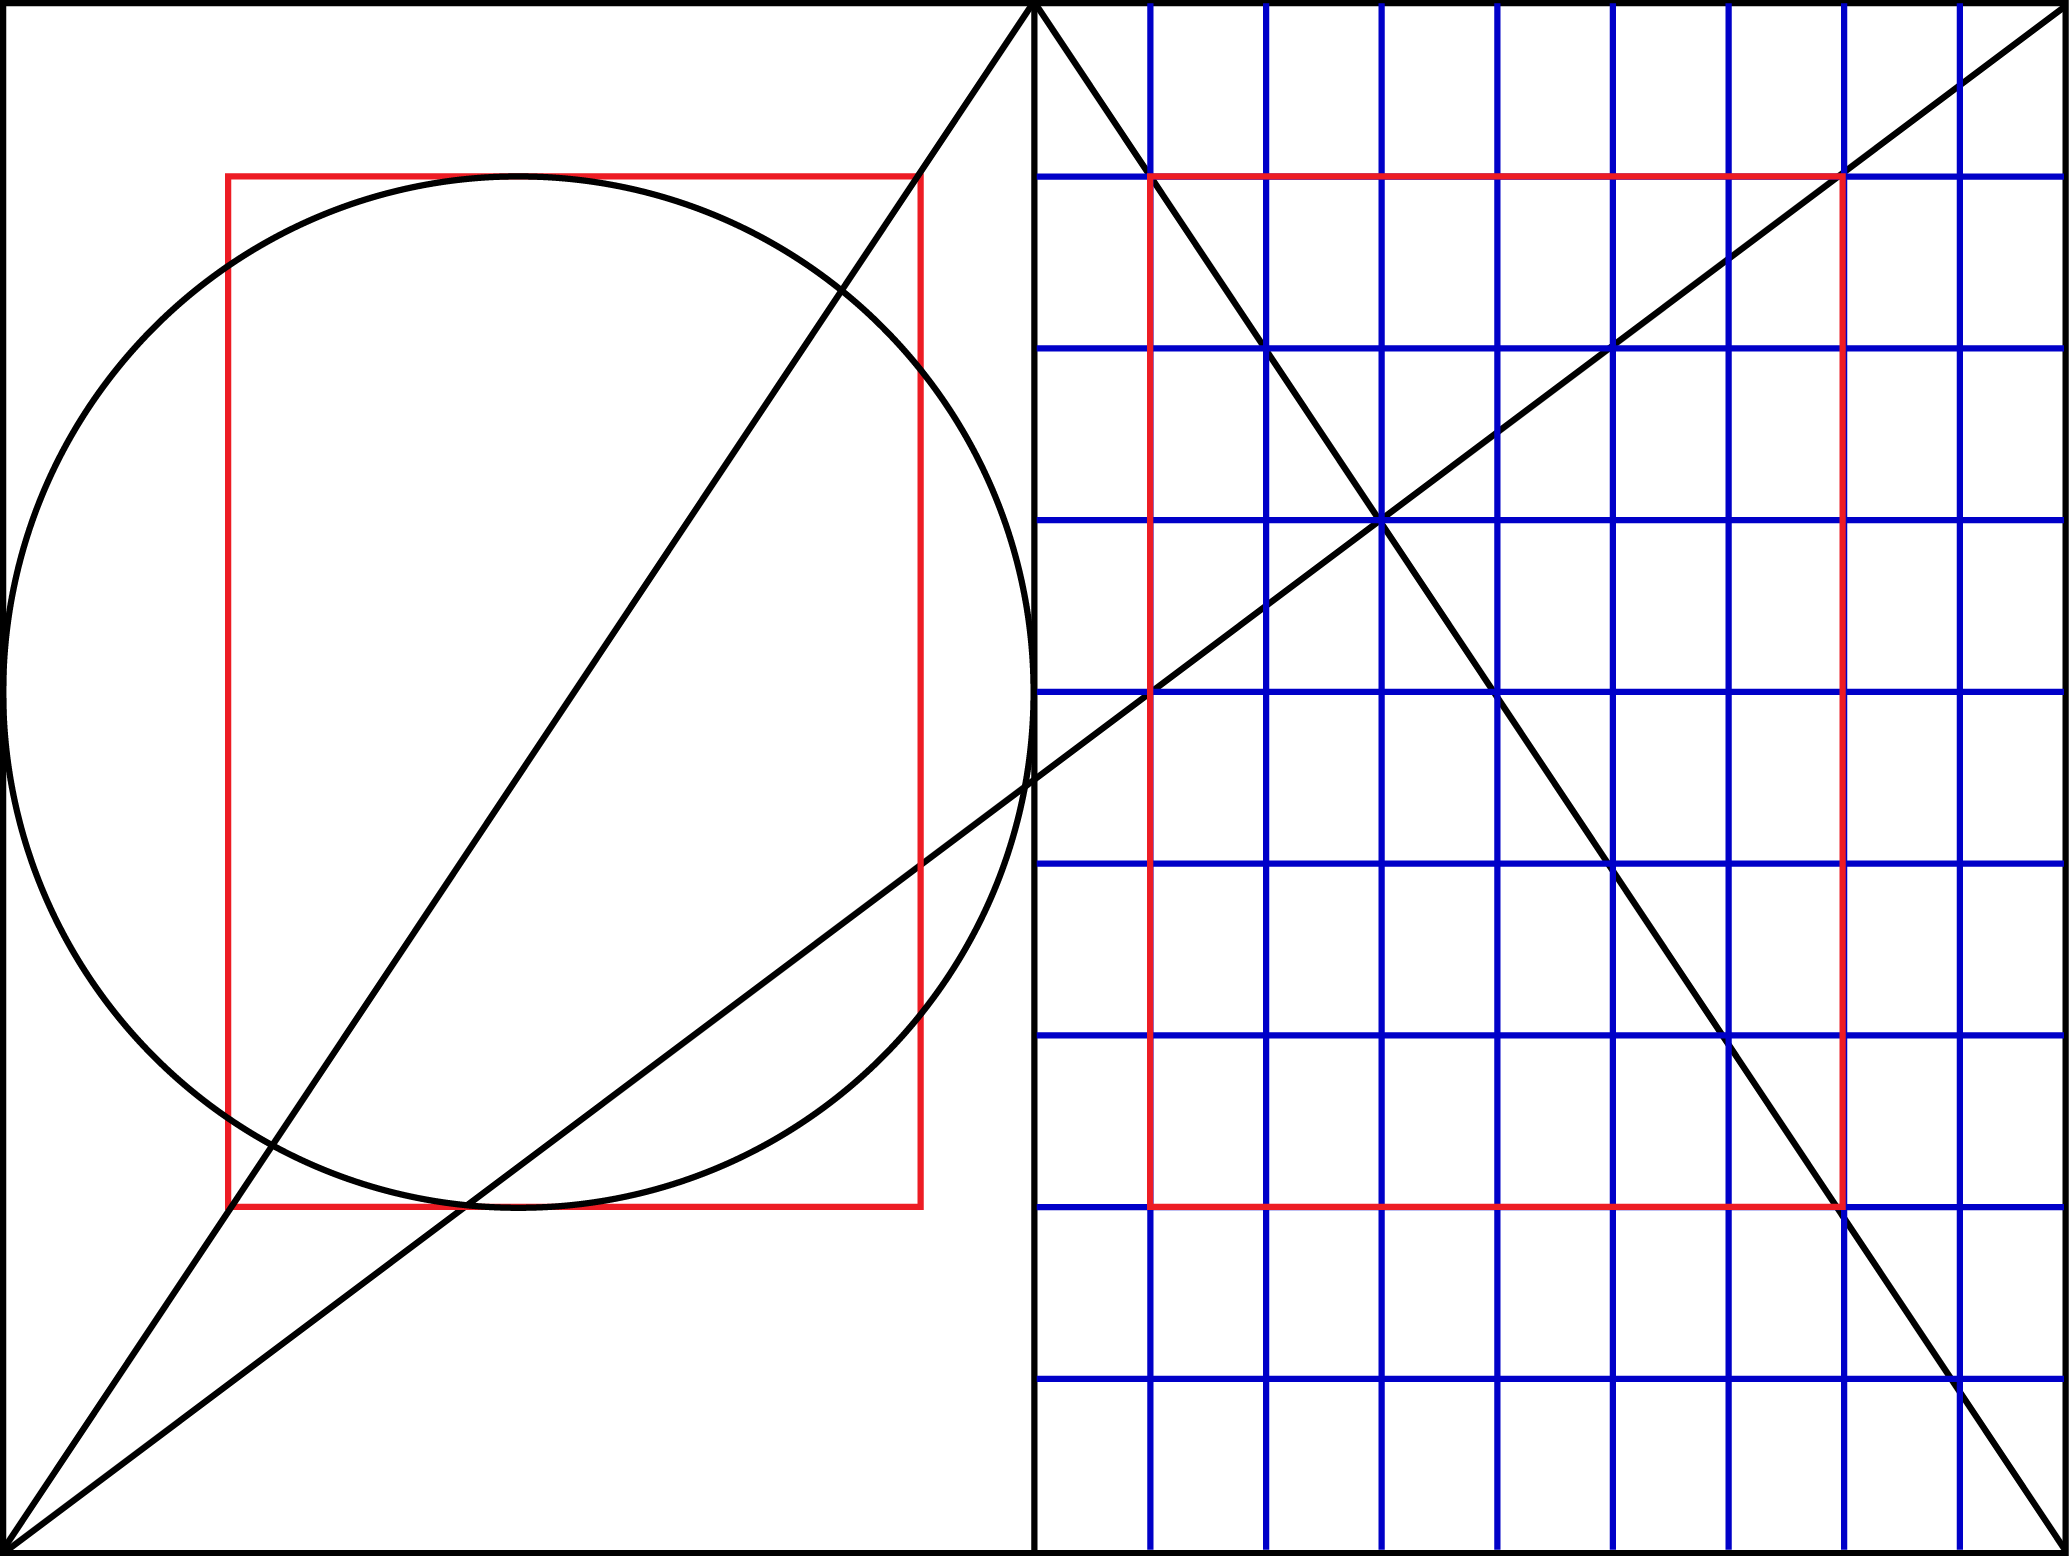
\includegraphics[width=0.4\textwidth]{Bilder/page_construction.png}
\caption{Satzspiegelkonstruktion nach Jan Tschichold (links) und Pául Rosarivo (rechts)}
\label{fig:TschicholdRosarivo}
\end{wrapfigure}

Lorem ipsum dolor sit amet, consetetur sadipscing elitr, sed diam nonumy eirmod tempor invidunt ut labore et dolore magna aliquyam erat, sed diam voluptua. At vero eos et accusam et justo duo dolores et ea rebum. Stet clita kasd gubergren, no sea takimata sanctus est Lorem ipsum dolor sit amet. Lorem ipsum dolor sit amet, consetetur sadipscing elitr, sed diam nonumy eirmod tempor invidunt ut labore et dolore magna aliquyam erat, sed diam voluptua. At vero eos et accusam et justo duo dolores et ea rebum. Stet clita kasd gubergren, no sea takimata sanctus est Lorem ipsum dolor sit amet.

\begin{wrapfigure}{r}{0.4\textwidth}
\hspace{-0.025\textwidth}
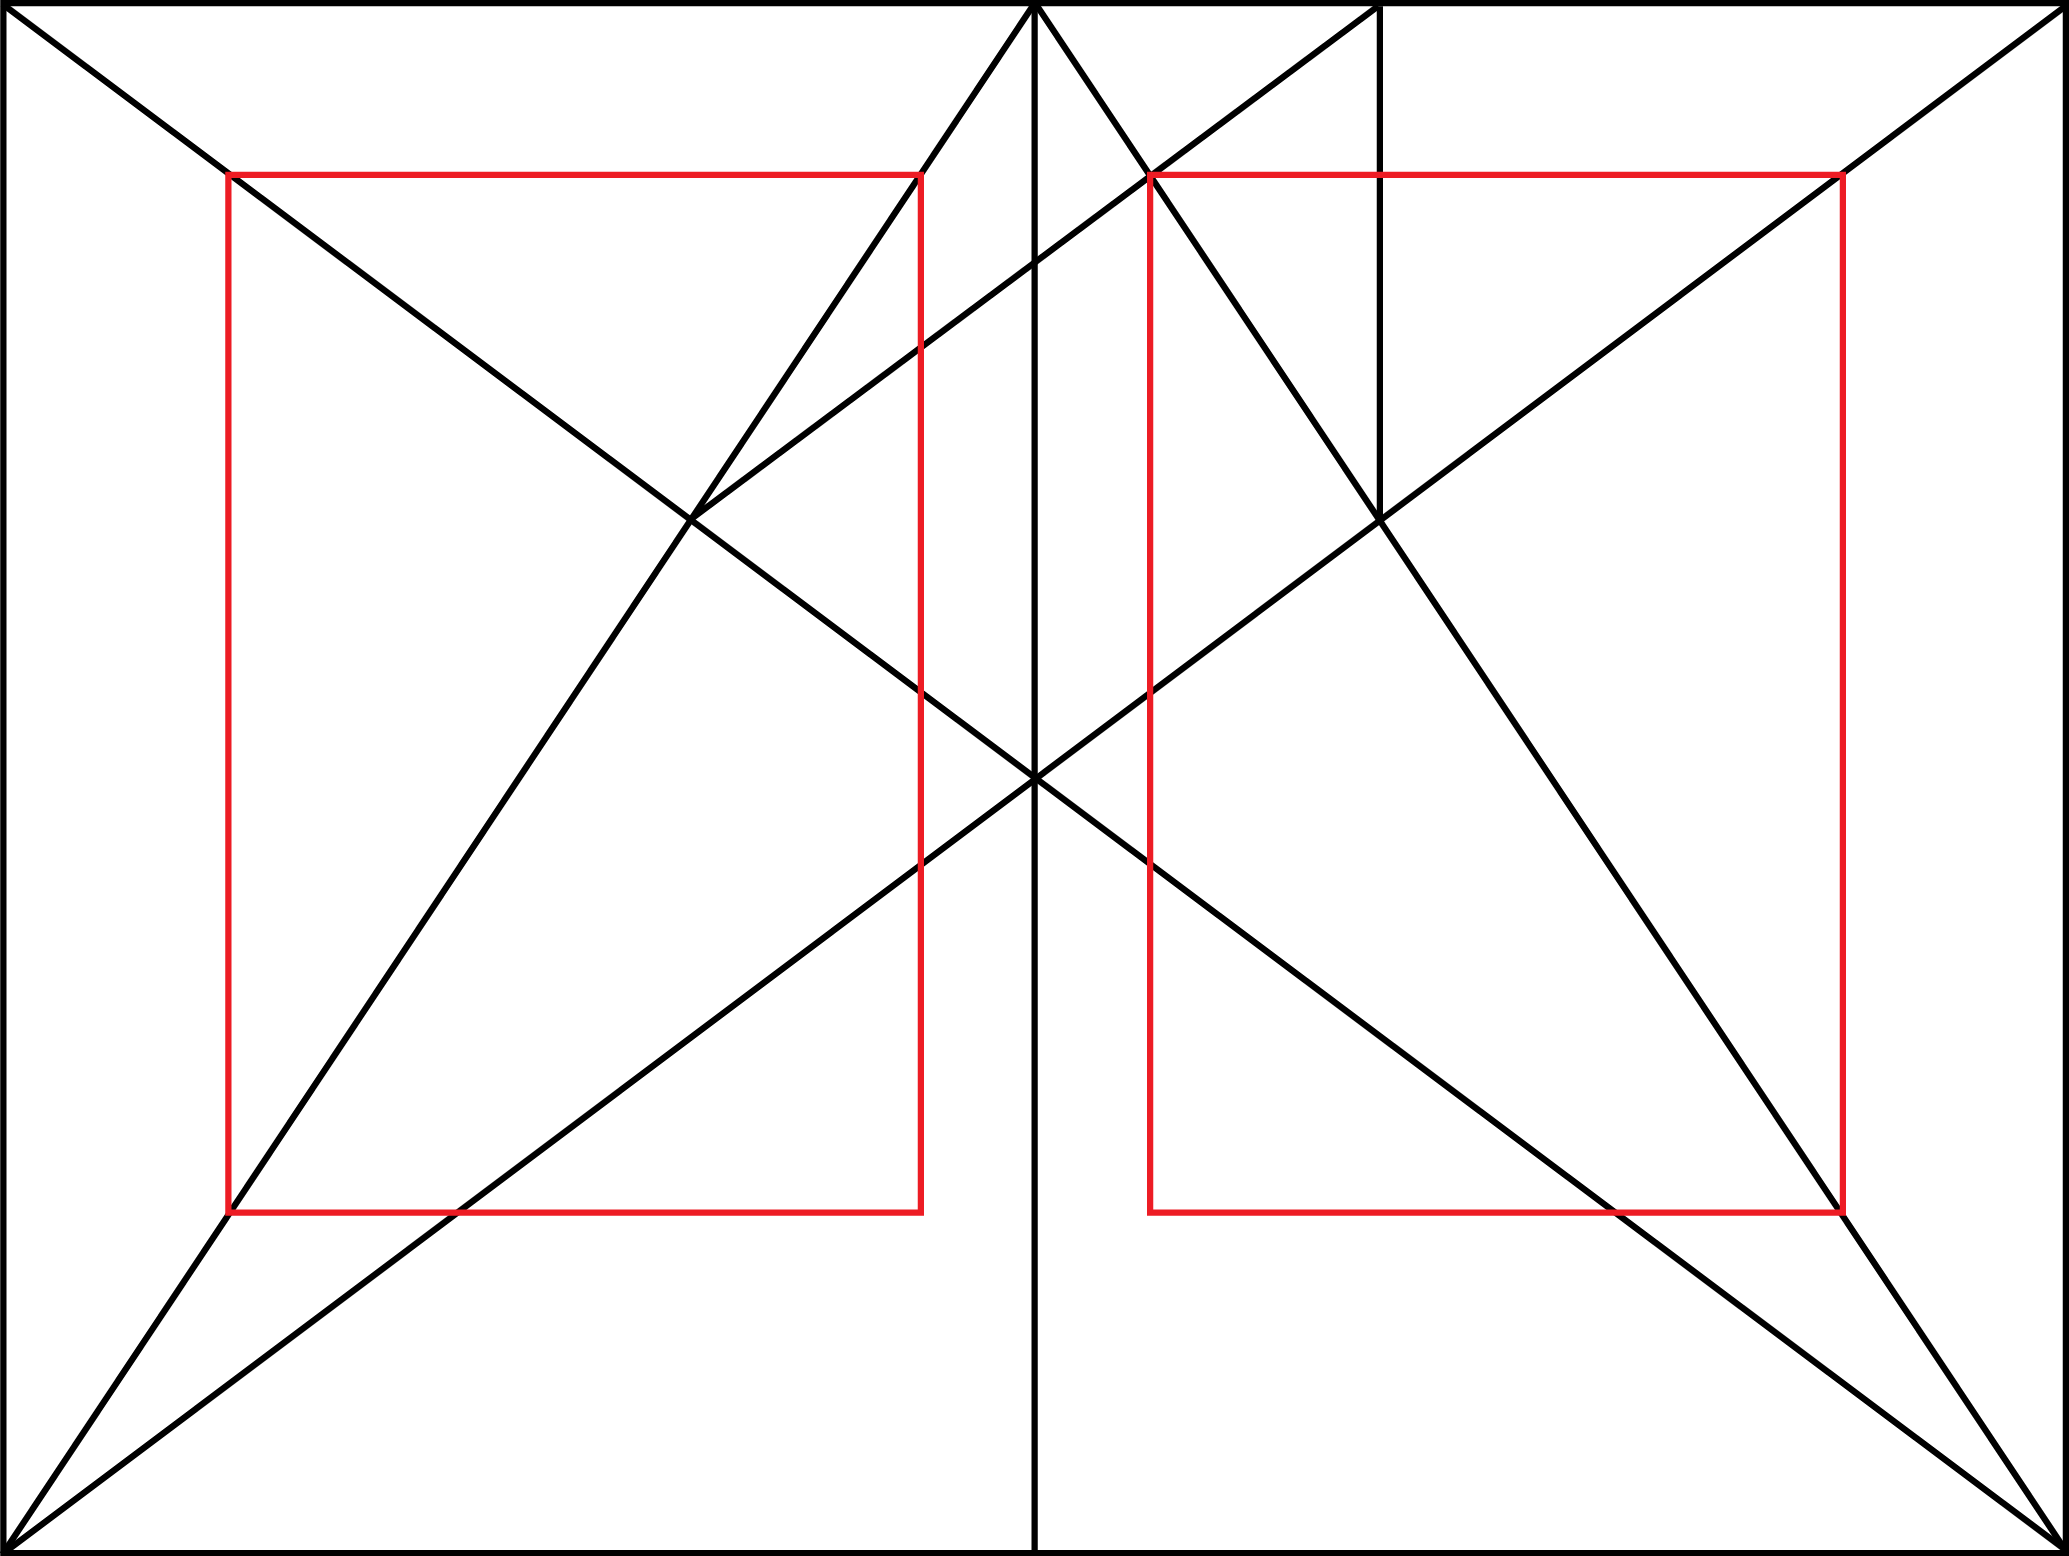
\includegraphics[width=0.4\textwidth]{Bilder/Van_de_Graaf_1.png}
\caption{Satzspiegel von Van de Graf}
\label{fig:VDG}
\end{wrapfigure}

Lorem ipsum dolor sit amet, consetetur sadipscing elitr, sed diam nonumy eirmod tempor invidunt ut labore et dolore magna aliquyam erat, sed diam voluptua. At vero eos et accusam et justo duo dolores et ea rebum. Stet clita kasd gubergren, no sea takimata sanctus est Lorem ipsum dolor sit amet. Lorem ipsum dolor sit amet, consetetur sadipscing elitr, sed diam nonumy eirmod tempor invidunt ut labore et dolore magna aliquyam erat, sed diam voluptua. At vero eos et accusam et justo duo dolores et ea rebum. Stet clita kasd gubergren, no sea takimata sanctus est Lorem ipsum dolor sit amet.

\begin{wrapfigure}{r}{0.4\textwidth}
\hspace{-0.025\textwidth}
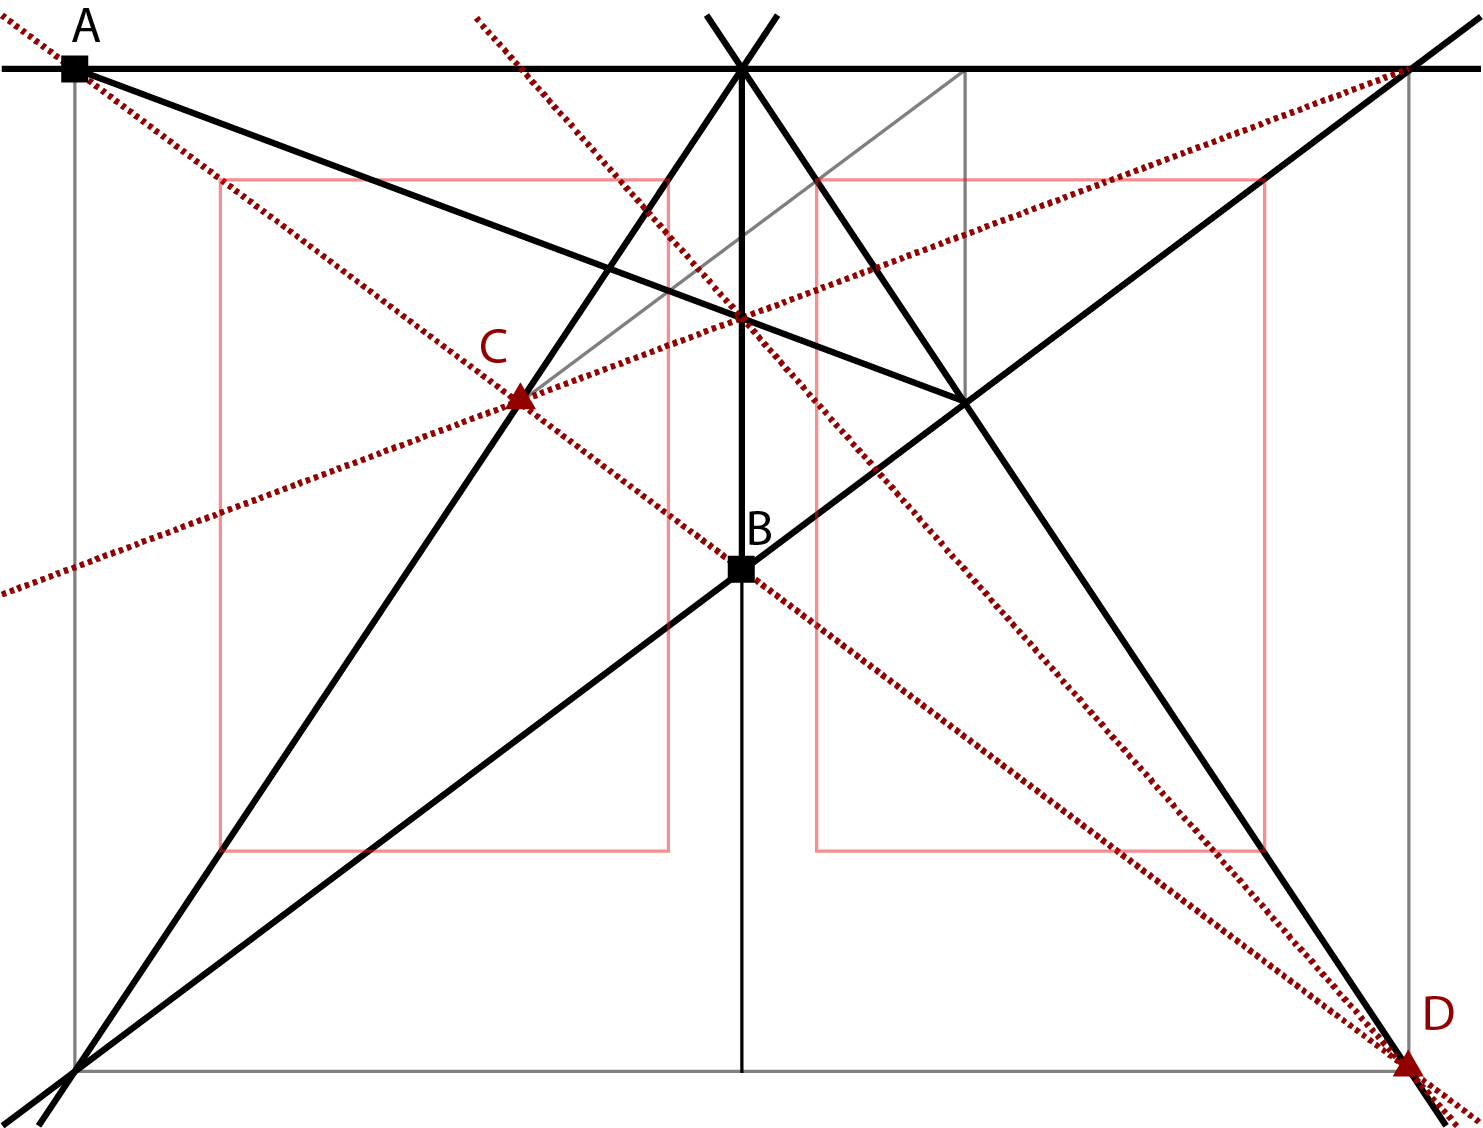
\includegraphics[width=0.4\textwidth]{Bilder/Van_de_Graaf.png}
\caption{Harmonische Lage im Satzspiegel}
\label{fig:harmVDG}
\end{wrapfigure}

Lorem ipsum dolor sit amet, consetetur sadipscing elitr, sed diam nonumy eirmod tempor invidunt ut labore et dolore magna aliquyam erat, sed diam voluptua. At vero eos et accusam et justo duo dolores et ea rebum. Stet clita kasd gubergren, no sea takimata sanctus est Lorem ipsum dolor sit amet. Lorem ipsum dolor sit amet, consetetur sadipscing elitr, sed diam nonumy eirmod tempor invidunt ut labore et dolore magna aliquyam erat, sed diam voluptua. At vero eos et accusam et justo duo dolores et ea rebum. Stet clita kasd gubergren, no sea takimata sanctus est Lorem ipsum dolor sit amet.


\begin{wrapfigure}{r}{0.4\textwidth}
\hspace{-0.025\textwidth}
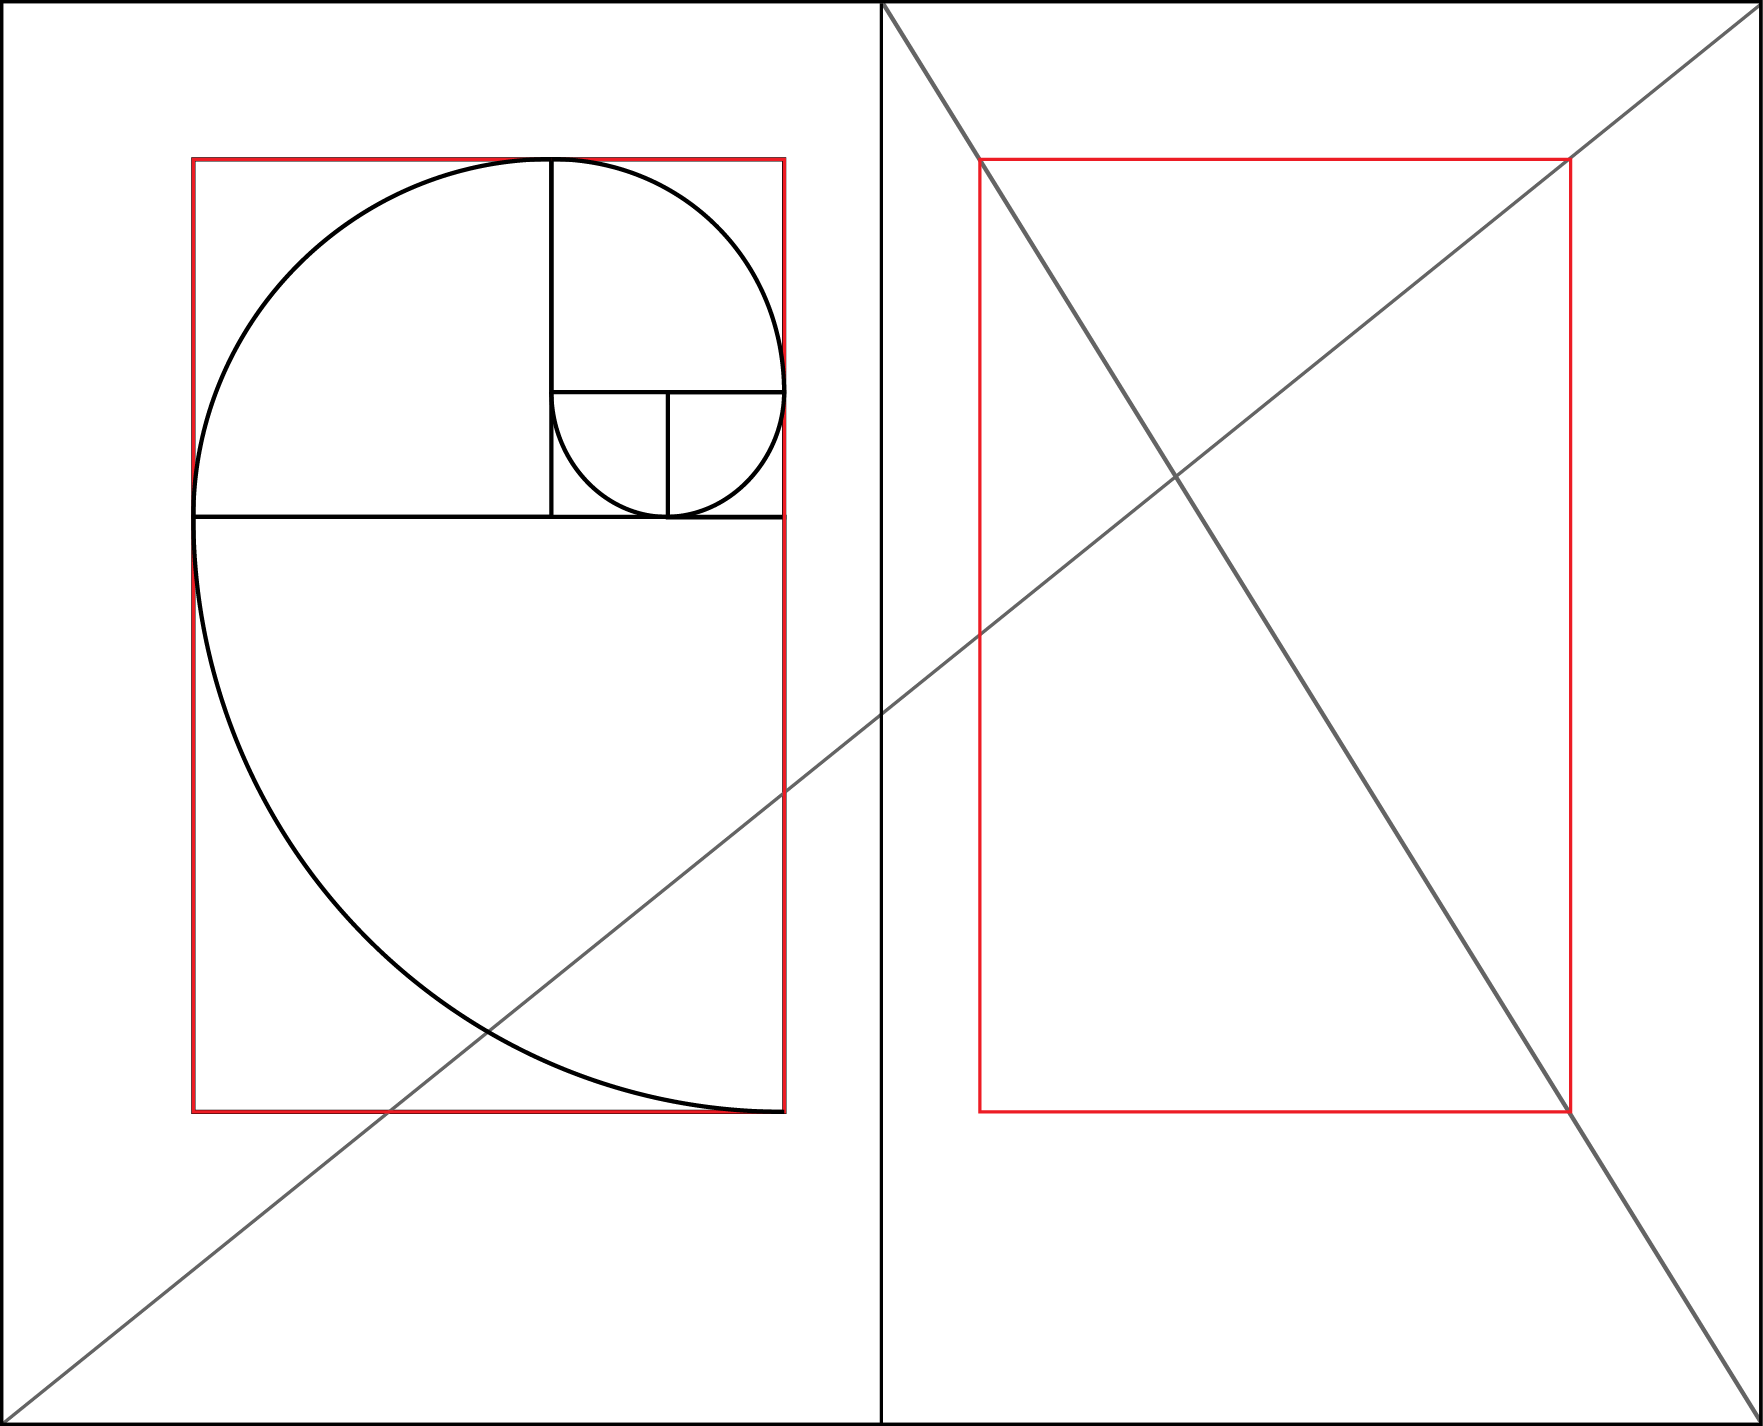
\includegraphics[width=0.4\textwidth]{Bilder/Golden_section_page_Tschichold.png}
\caption{Satzspiegel von Tschichold nach Fibonacci-Folge ausgelegt}
\label{fig:fibSatz}
\end{wrapfigure}

Lorem ipsum dolor sit amet, consetetur sadipscing elitr, sed diam nonumy eirmod tempor invidunt ut labore et dolore magna aliquyam erat, sed diam voluptua. At vero eos et accusam et justo duo dolores et ea rebum. Stet clita kasd gubergren, no sea takimata sanctus est Lorem ipsum dolor sit amet. Lorem ipsum dolor sit amet, consetetur sadipscing elitr, sed diam nonumy eirmod tempor invidunt ut labore et dolore magna aliquyam erat, sed diam voluptua. At vero eos et accusam et justo duo dolores et ea rebum. Stet clita kasd gubergren, no sea takimata sanctus est Lorem ipsum dolor sit amet.

\subsubsection{Gestaltungsraster}

\newpage
\section{Zusammenfassung}

\newpage
\listoffigures

\newpage
\nocite{proCG}
\nocite{perspectivesOnProGeo}
\nocite{doppelVerhaeltnis}
\nocite{proGeoGrundlagen}
\addcontentsline{toc}{section}{Literaturverzeichnis}
\bibliography{Harmonische_Lage}
\bibliographystyle{plain}


\end{document}